

% code=utf-8
\documentclass[UTF8]{ctexart}
\usepackage{amsmath}
\usepackage{graphicx}
\begin{document}

\section{数列敛散性}
数列收敛于A,则任意子数列收剑于A   \\
单调数列的某一子数列收敛于A,则该数列收敛于A \\
数列{2n}与{2n+1}都收敛于A,则数列必收敛于A

\section{连续的定义}
$$ \lim_{x\rightarrow a}f(x)=A$$
$$ \lim_{\Delta\rightarrow0}\Delta y=\lim_{\Delta x \rightarrow 0 } f(x+ \Delta x) - f(x)=0$$

\section{常用等价无穷小}
 $ x \rightarrow 0$
$ \sin x \sim x$ ; $ \tan x \sim x$ ; $ \arcsin x \sim x$ ; $ \arctan x \sim x$ ; $ \ln({1+x}) \sim x $ ; $ e^x -1 \sim x$ ; $ a^x -1 \sim x \ln a $ ; $ 1-\cos x \sim \frac{1}{2} x^2 $ ; $ {(1+x)}^a -1 \sim ax$ \\

f(0)=1 时 等价无穷小 \\
$$ \lim_{x \rightarrow 0 } {{\int_0^x f(x)dt} \over {x}} =1$$

$$ \lim_{x \rightarrow 0} x \ln x =0$$
$$\lim_{t \rightarrow 0} t e^t =0 $$
$$\lim _{x \rightarrow 0^+} x^x =1$$
$$(x^x)'=x^x(1+ \ln x)$$

\section{极限比较}
$$ f(x) \geq g(x) \rightarrow \lim f(x) \geq \lim g(x) $$
$$ \lim f(x) > \lim g(x) \rightarrow f(x) > g(x) $$
\section{敛散}
$ \lim_{x \rightarrow 1} \frac{1}{(x-1)^{α+1}}=
  \begin{cases}
  &0 , (a<-1) \\
  &1 , (a=-1) \\
  &\infty ,(a>-1)
\end{cases}
$
$$ \frac{\partial f}{\partial x} \equiv \frac{\partial f}{\partial y} \equiv 0\ \leftrightarrow df({x,y}) \equiv 0 $$

\section{基本函数求导公式}
$ (a^x)'=a^x \ln a \\
  ( \log _a x)'=\frac{1}{x \ln a} $

\section{球体积\&表面积}
$$ V=\frac{4}{3} \pi R^3$$
$$ S= 4 \pi R^2$$

\section{定积分定义}
$$ \int_a^b f(x)dx= \lim_{n \rightarrow \infty } \sum_{i=1}^n \frac{f \left( a+ \frac{b-a}{n}i \right)(b-a)}{n}$$
\section{连续函数必有原函数}
含有第一类间断点,无穷间断点的函数在包含间断点的区间没有原函数   \\
跳跃间断点可以有原函数 \\

\section{基本积分表}
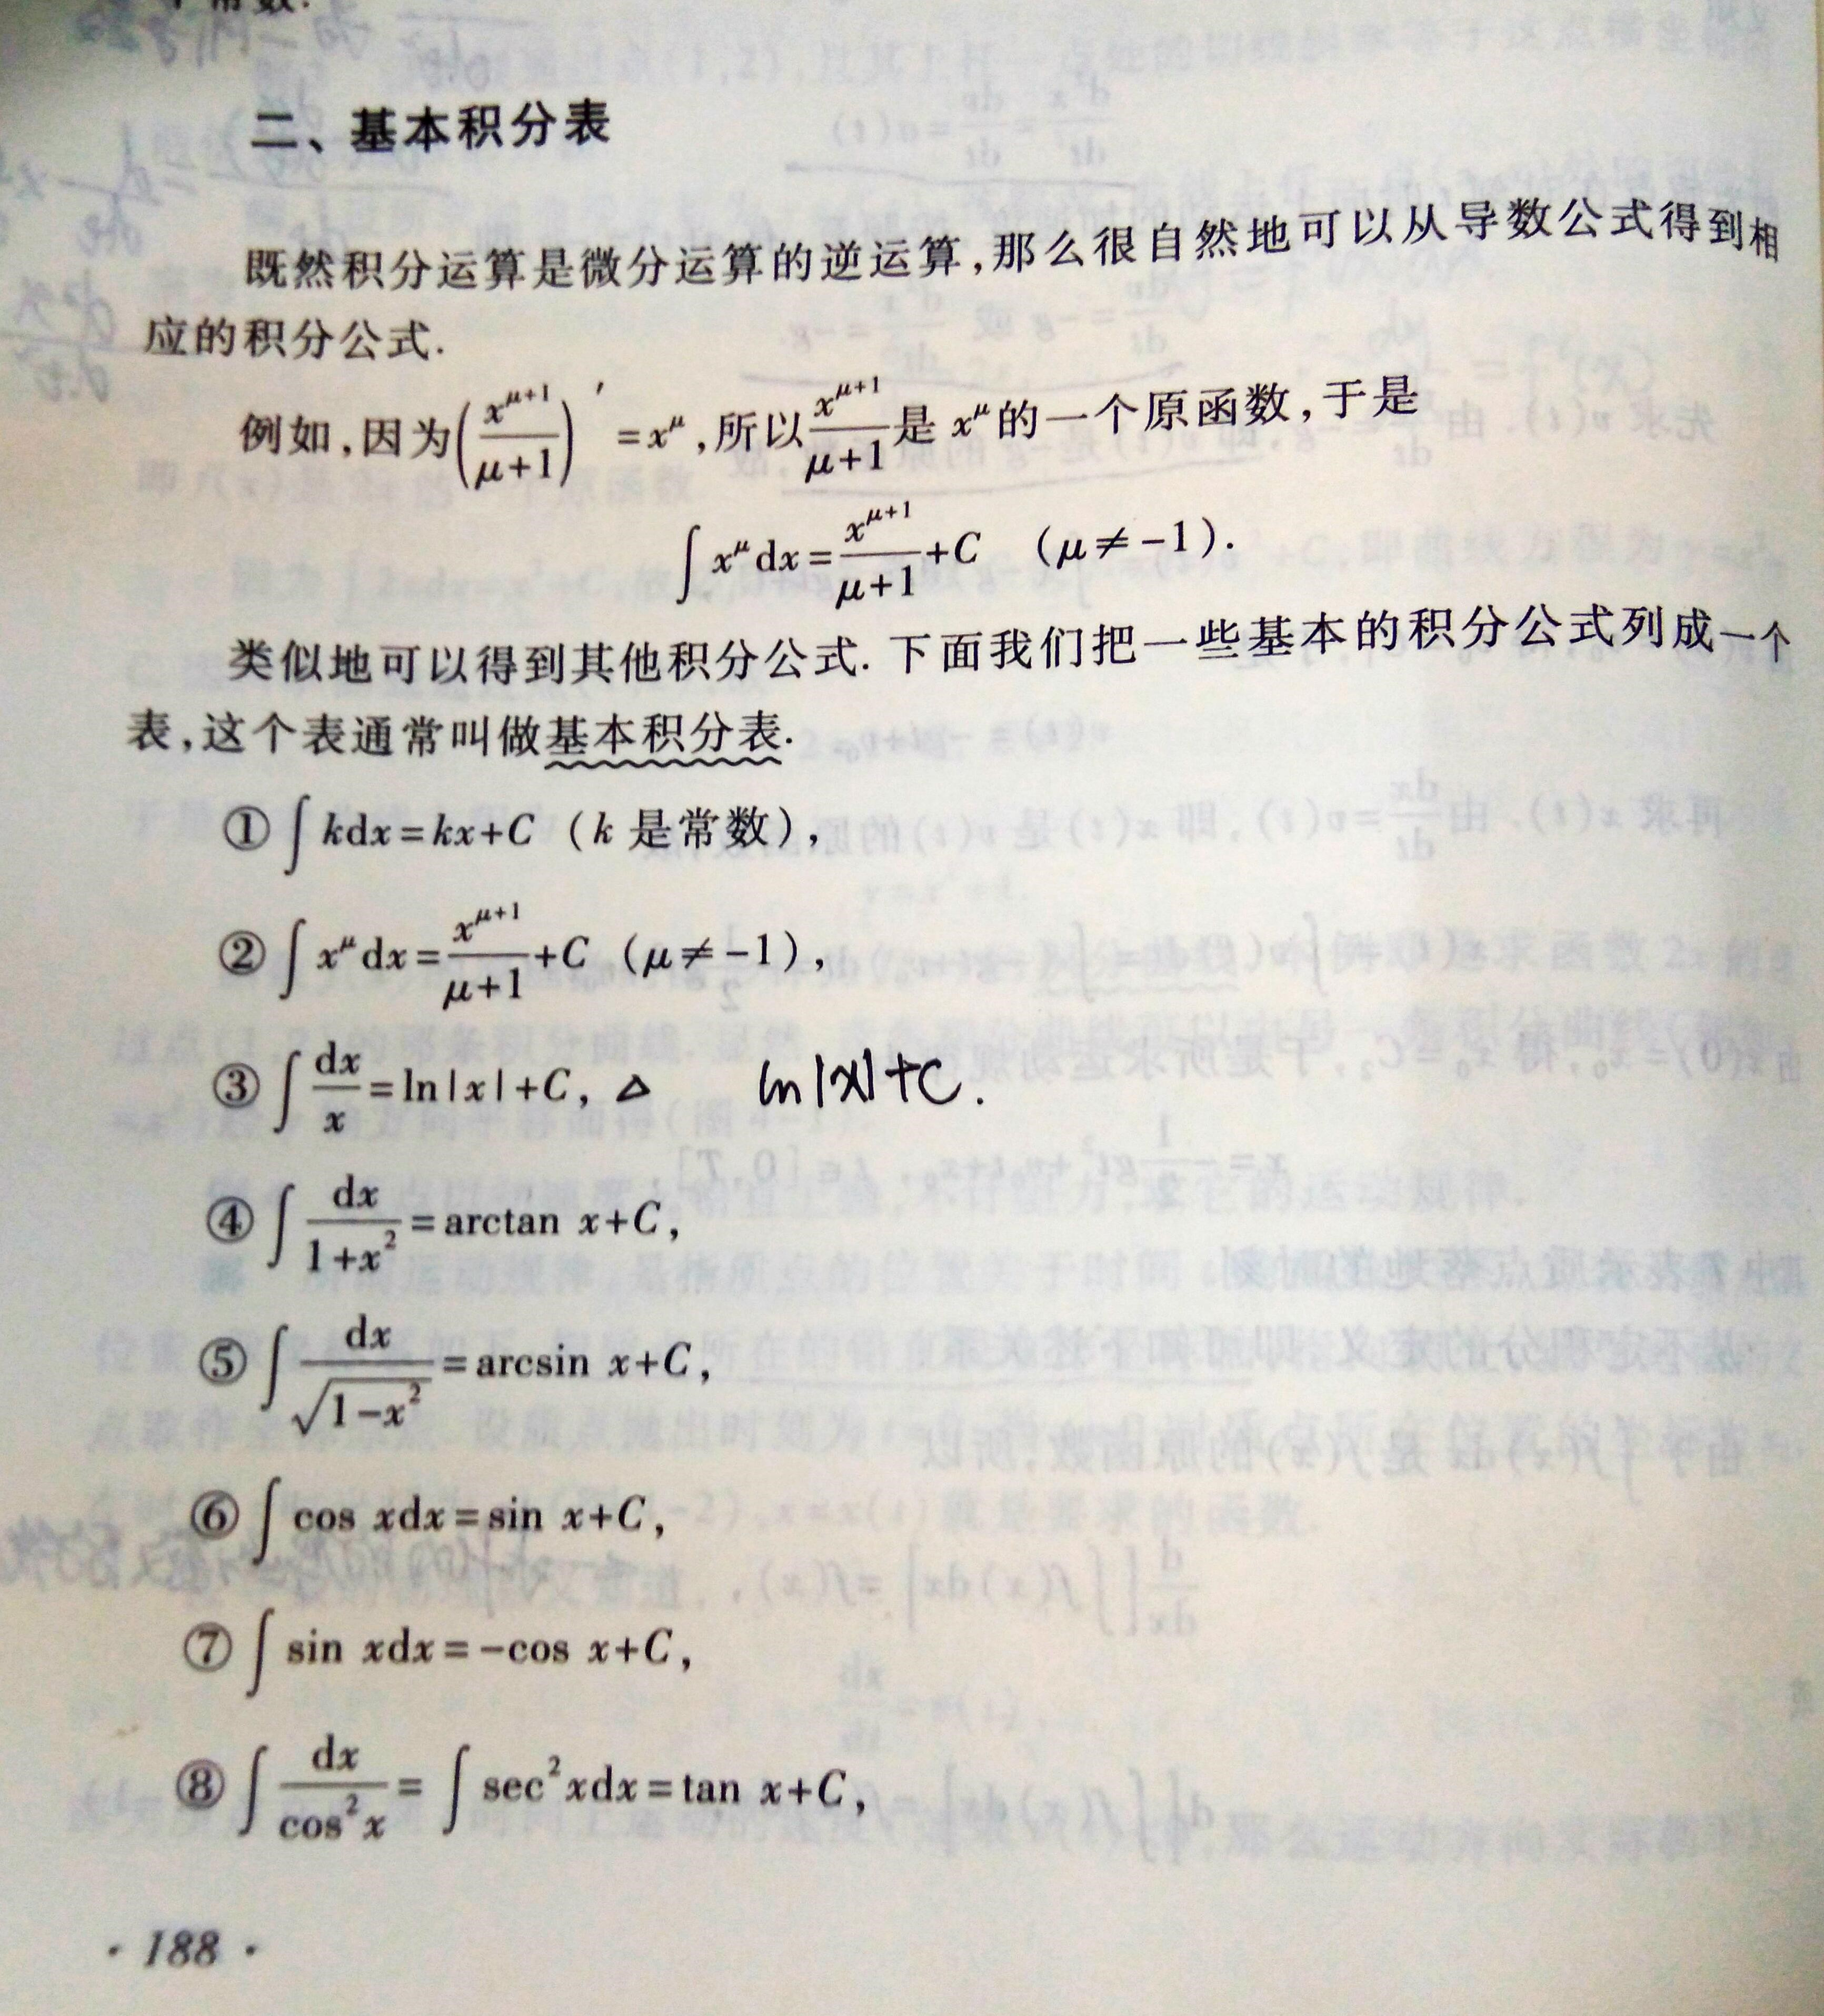
\includegraphics[width=14cm]{9345E7/9476215E0863B8FB681EC9D2BB921BDB.jpg}
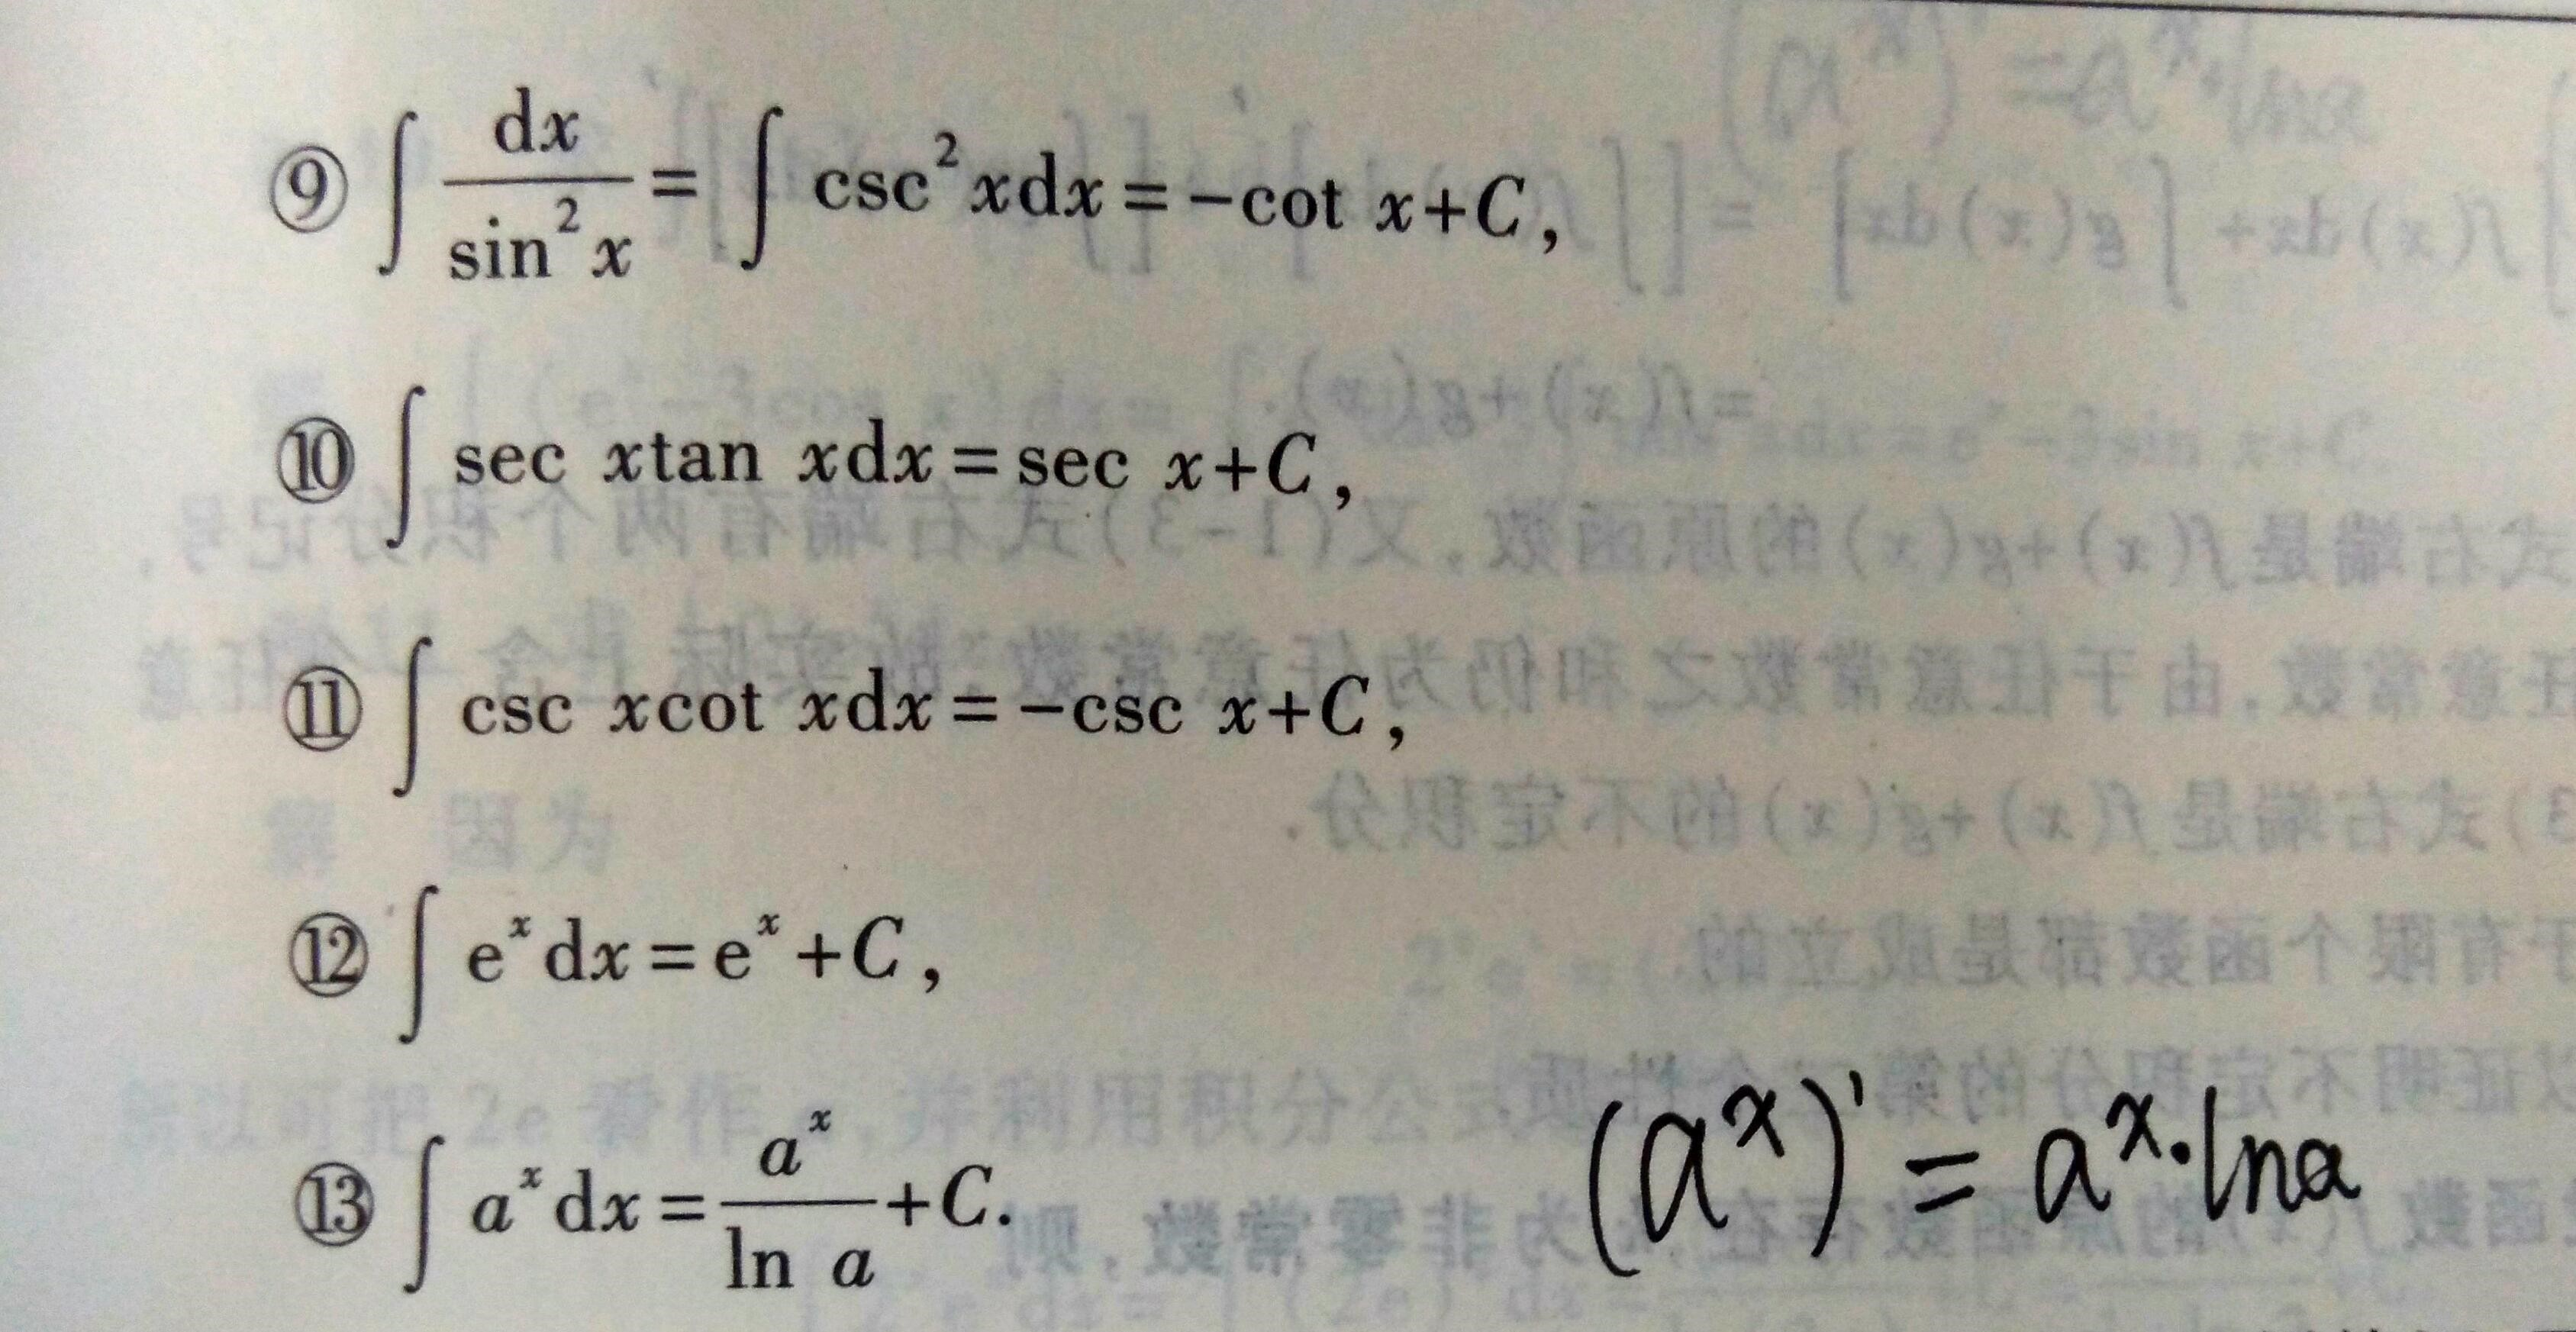
\includegraphics[width=14cm]{9345E7/4FEE9C843E57935F87D1E16F255FA43E.jpg}

$$=\int \frac{\cos t dt}{\sin t + \cos t} \\
=\frac{1}{2} \int \frac{\cos t + \sin t +\cos t - \sin t}{\sin t + \cos t}dt \\
= \frac{1}{2} + \frac{1}{2} \ln | \sin t + \cos t| +C $$

当 x=a+b-t \\
$ \int_a^b f(x) dx = \int_b^a f(a+b-t)d(a+b-t)=\int_a^bf(a+b-t)dt=\int_a^b f(a+b-x) dx \\
\int_a^b f(x) dx = \frac{1}{2} [ f(x) + f(a+b-x) ] dx$

$$ \int \tan x dx = - \ln |\cos x | +C$$
$$ \int cot x dx = \ln|\sin x| +C$$
$$ \int \sec x dx = \ln |\sec x+ \tan x| +C$$
$$ \int \csc x dx = \ln|csc x-\cot x | +C $$
$$ \int \frac{dx}{a^2+x^2}=\frac{1}{a} \arctan \frac{x}{a} +C $$
$$ \int \frac{dx}{x^2-a^2}=\frac{1}{2a} \ln \left| \frac{x-a}{x+a} \right| +C$$
$$ \int \frac{dx}{\sqrt{a^2-x^2}}=\arcsin \frac{x}{a}+C$$
$$ \int \frac {dx}{\sqrt{x^2+a^2}}=\ln {(x+ \sqrt{x^2+a^2})}+C$$
$$ \int \frac{dx}{\sqrt{x^2-a^2}}= \ln | x+\sqrt{x^2-a^2}|+C$$

\section{泰勒公式}
$ e^{1+x}=e+ex+e \frac{x^2}{2!} + e \frac{x^3}{3!}+e\frac{x^4}{4!}$ \\
$ (1+x)^{\frac{1}{x}} \sim e-\frac{e}{2}x+\frac{11}{24}ex^2+o(x^2)$ \\
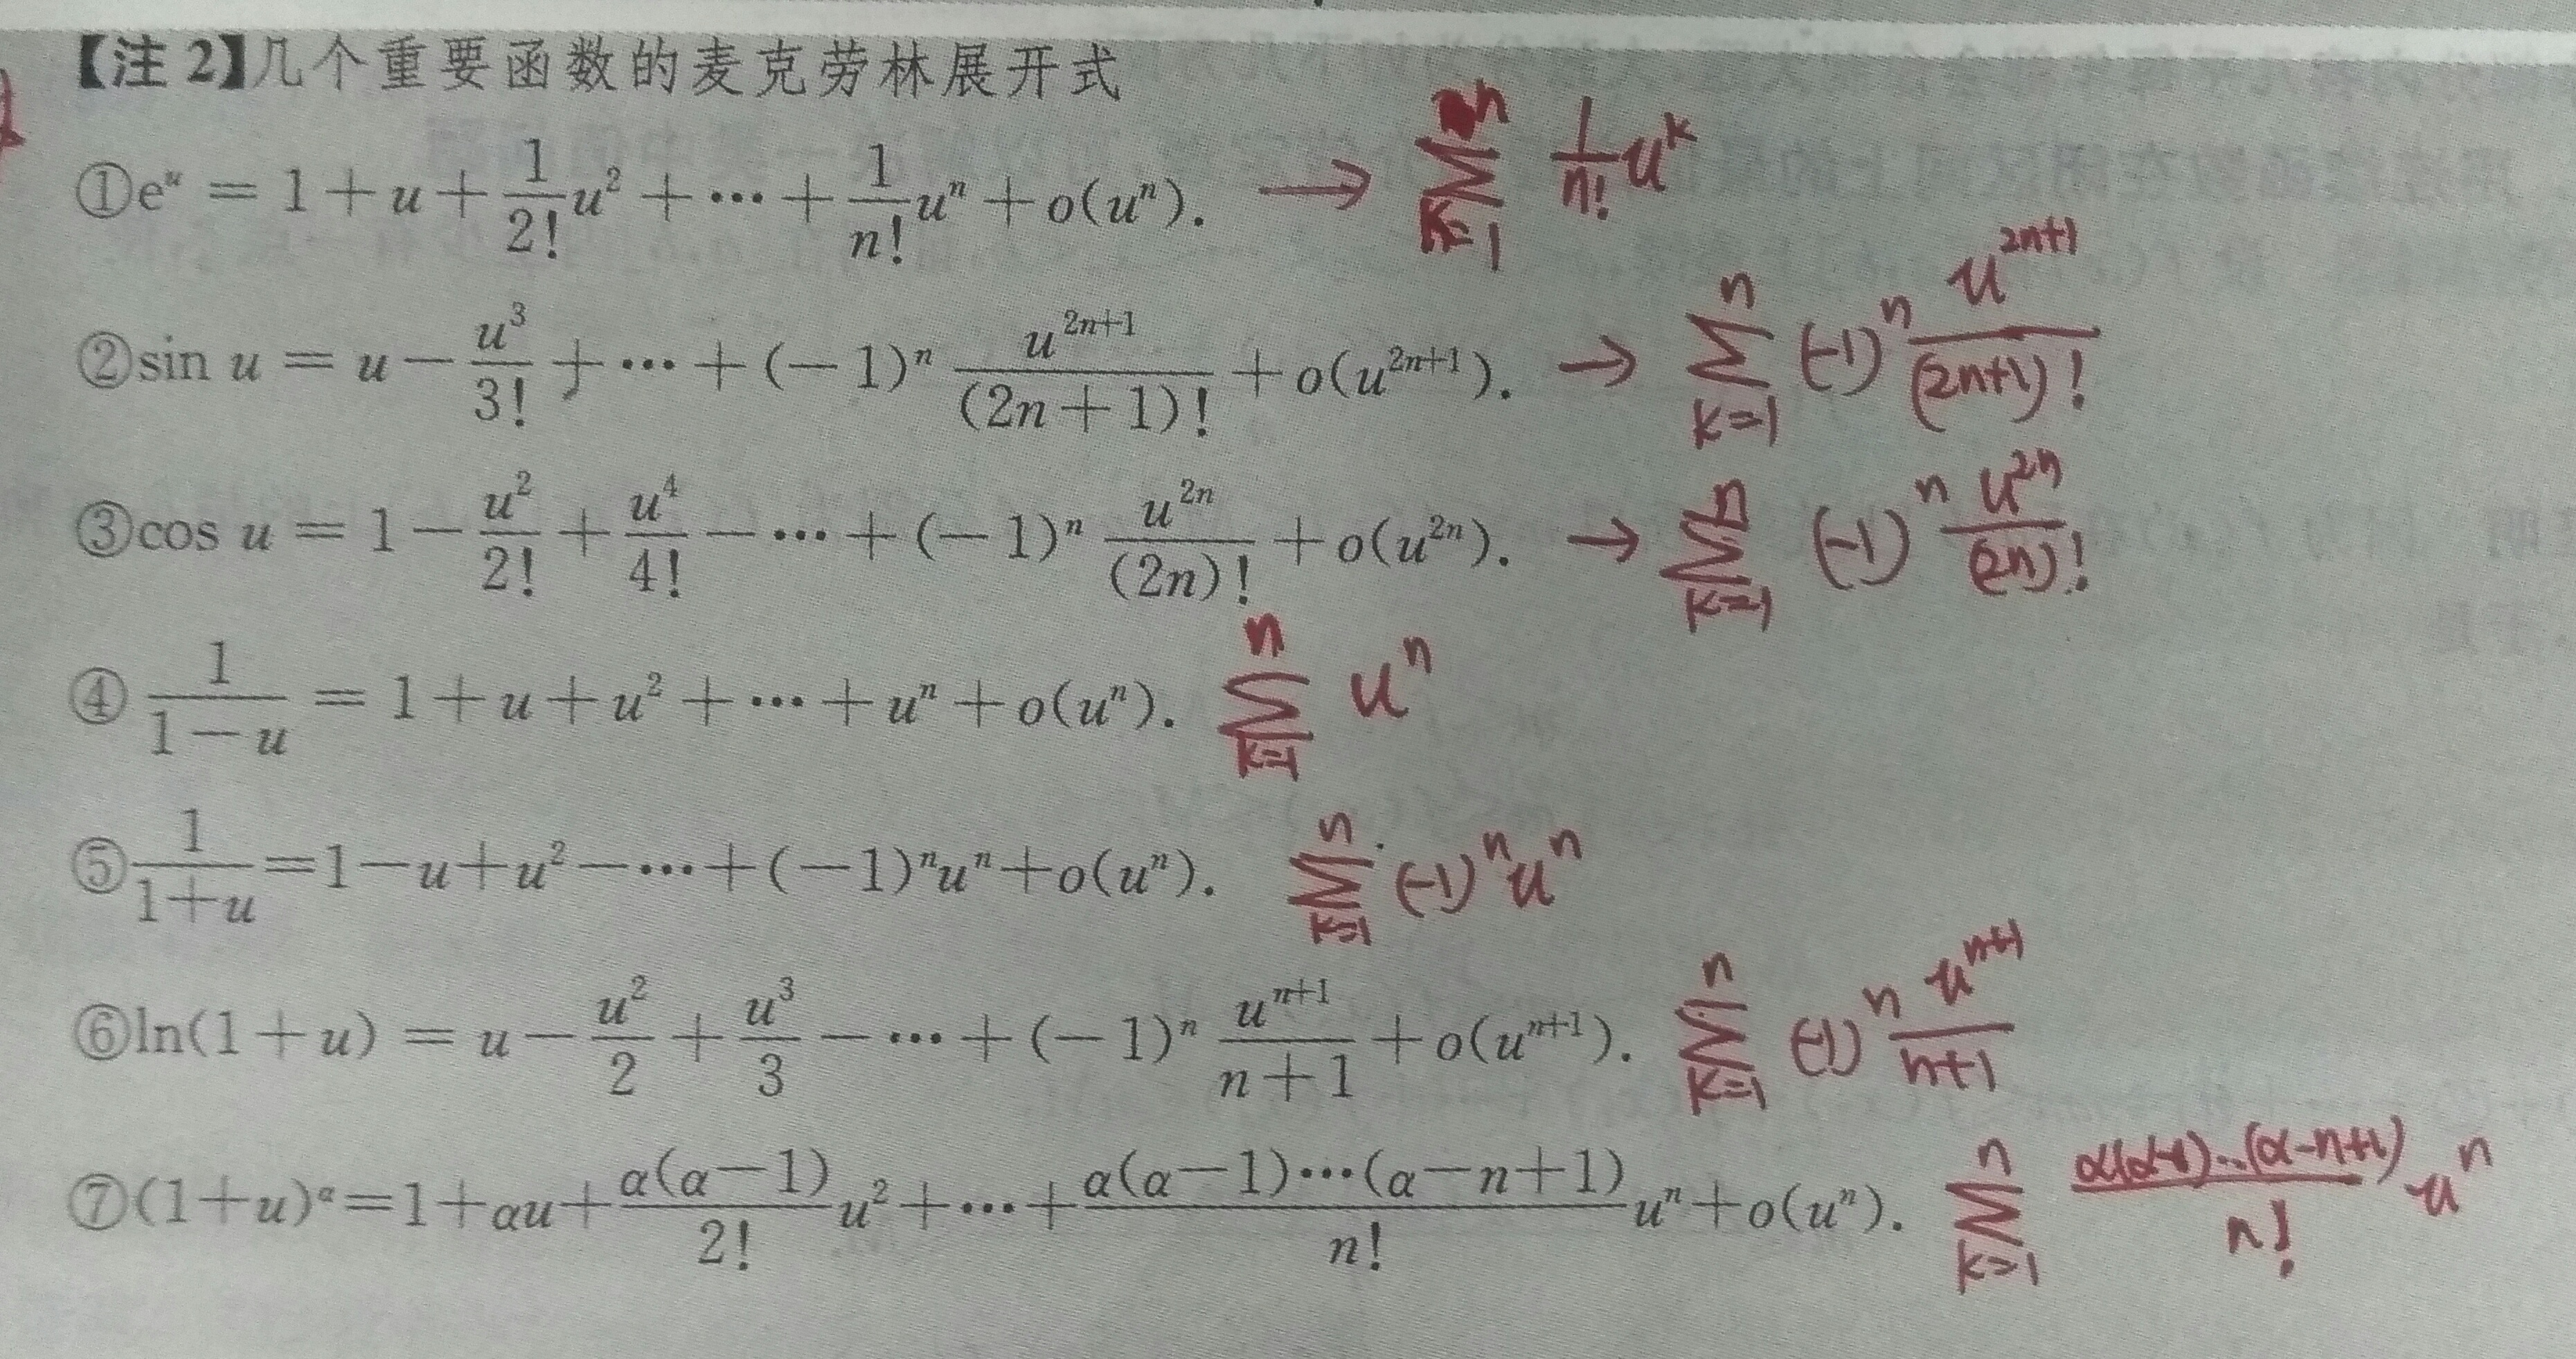
\includegraphics[width=14cm]{9345E7/F04F85A8EB6EABFF18D6BE71383F2472.jpg}
$$ \sin x=x-\frac{x^3}{3!}+o(x^3)$$
$$ \cos x=1-\frac{x^2}{2!}+\frac{x^4}{4!}+o(x^4)$$
$$ \arcsin x=x+\frac{x^3}{3!}+o(x^3)$$
$$ \tan x=x+\frac{x^3}{3}+o(x^3)$$
$$ \arctan x=x-\frac{x^3}{3}+o(x^3)$$

\section{几个初等函数的n阶导数公式}
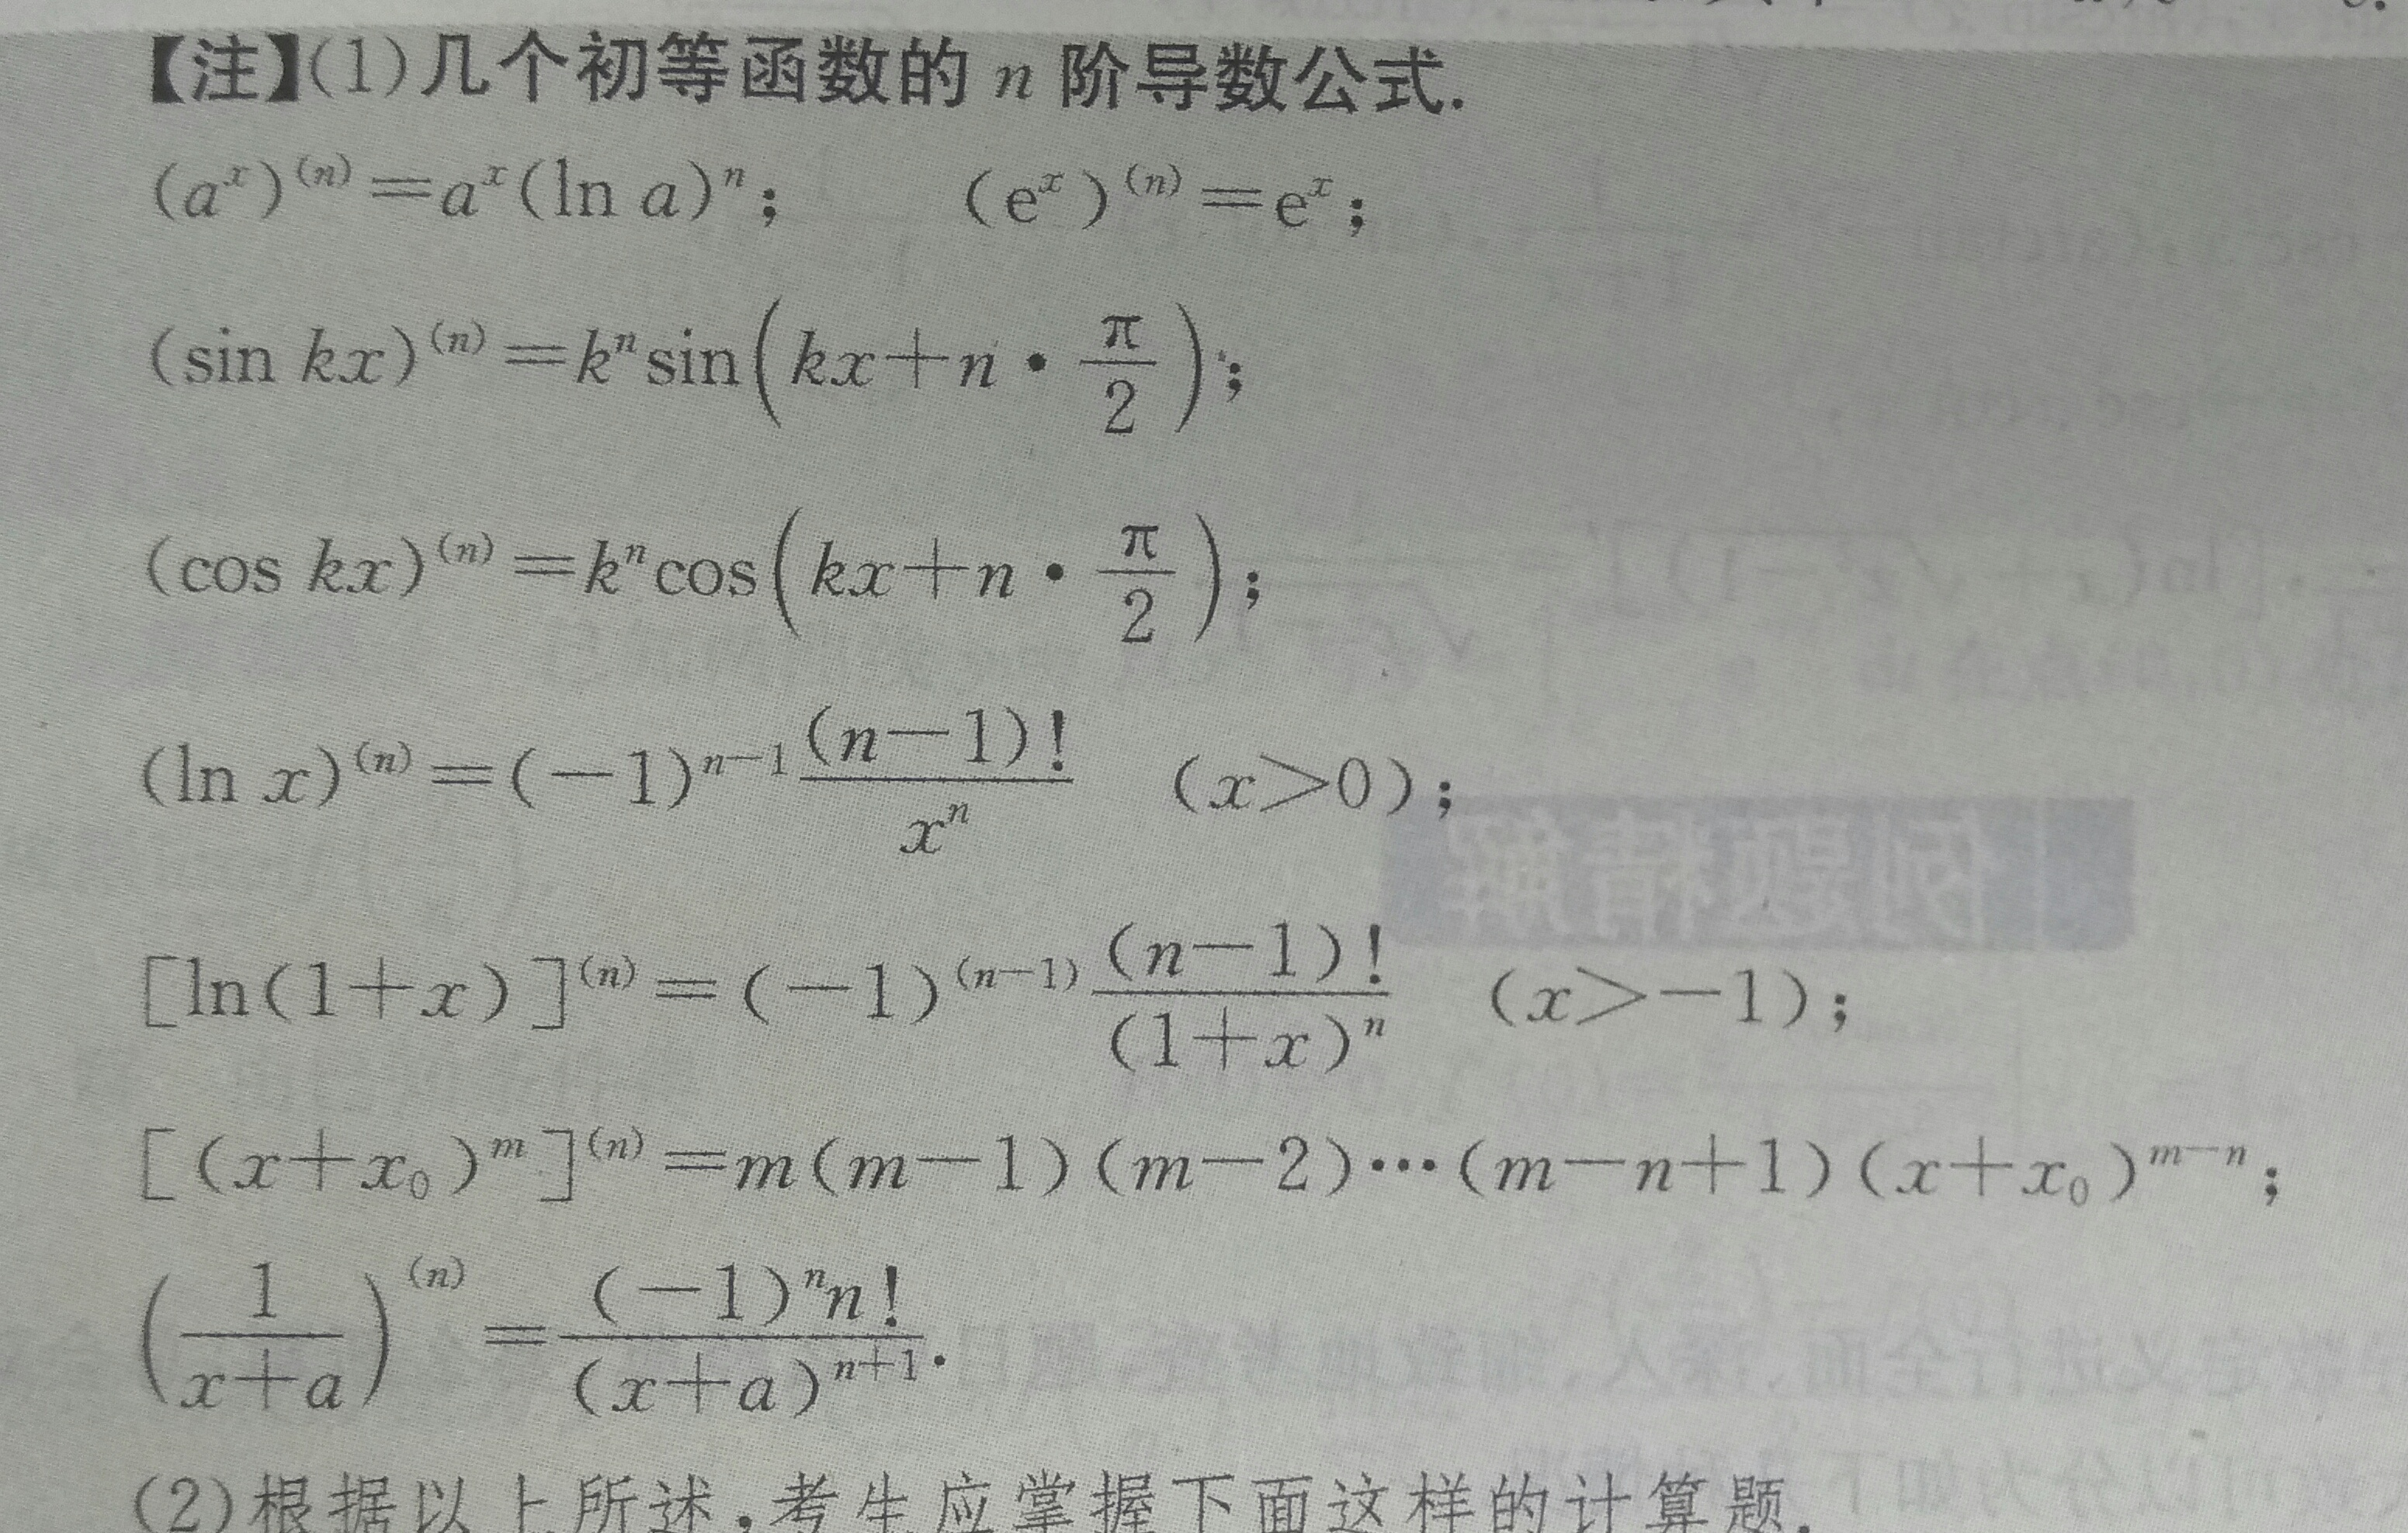
\includegraphics[width=13cm]{9345E7/2A793F093B002F668B144F9ED087EB77.jpg}


$$ \int_0^\frac{\pi}{2} sin^n θ d \theta =\int_0^\frac{\pi}{2} \cos^n \theta d \theta =
\begin{cases}
  &\frac{n-1}{n}\cdot\frac{n-3}{n-2} \cdots \frac{3}{4}\cdot\frac{1}{2}\cdot\frac{\pi}{2}\mbox{  n为正偶数} \\
  &\frac{n-1}{n}\cdot\frac{n-3}{n-2}\cdots\frac{4}{5}\cdot\frac{2}{3}\mbox{  n为大于1的正奇数}
\end{cases}
$$

\section{经典不等式}
$$e^x \geq x+1 ; x-1 \geq \ln x ; \frac{1}{1+x} < \ln \left( 1+ \frac{1}{x} \right) < \frac{1}{x}$$
$$ e^{αx} \gg x^b \gg \ln^y x $$
$$ 2\left| ab \right| \leq a^2+b^2$$
$$ \left| a \pm b \right| \leq |a|+|b|$$
$$ \left| |a| - |b| \right| \leq |a-b|$$
$$\sqrt{ab} \leq \frac{a+b}{2} \leq \sqrt{\frac{a^2+b^2}{2}}$$
当 x>0,y>0,p>0,q>0,$\frac{1}{p}+\frac{1}{q}=1 \rightarrow xy \leq \frac{x^p}{p}+\frac{y^q}{q}$
$$(a^2+b^2)(c^2+d^2) \geq (ac+bd)^2$$
$$ [\int_a^b f(x)g(x)dx]^2 \leq \int_a^b f^2(x)dx\cdot \int_a^b g^2(x)dx$$
$$\mbox{当} p>1, \frac{1}{p}+\frac{1}{q}=1 \mbox{时;} \left| \int_a^b f(x) \cdot g(x)dx\right| \leq \left[ \int_a^b \left| f(x) \right|^p dx \right] ^\frac{1}{p} \cdot \left[ \int_a^b \left| g(x) \right|^q dx \right] ^\frac{1}{q}$$

\section{定理}
​若$\int^{(n-1)}(x)$最多只有一个实零点,则f(x)最多只有n个不同实零点 \\
$f^′(x)≠0$ 且连续⇒ f(x)单调 \\
连续的**奇**函数的**一  切**原函数都是**偶**函数 \\
连续的**偶**函数的**仅有一个**原函数都是**奇**函数 \\
可积函数在区间内必有界 (二元也成立) \\
f(x)是以ㄒ为周期的可积函数 \\

\section{常见正弦积分}

$$ \int_0^\frac{\pi}{4} \sin x dx =1- \frac{\sqrt{2}}{2}$$
$$ \int_\frac{\pi}{4}^\frac{\pi}{2} \sin x dx =\frac{\sqrt{2}}{2}$$
$$ \int_0^\frac{\pi}{2} \sin x dx = 1$$
$$ \int_0^\pi \sin x dx =2$$

\section{积分递归解法}
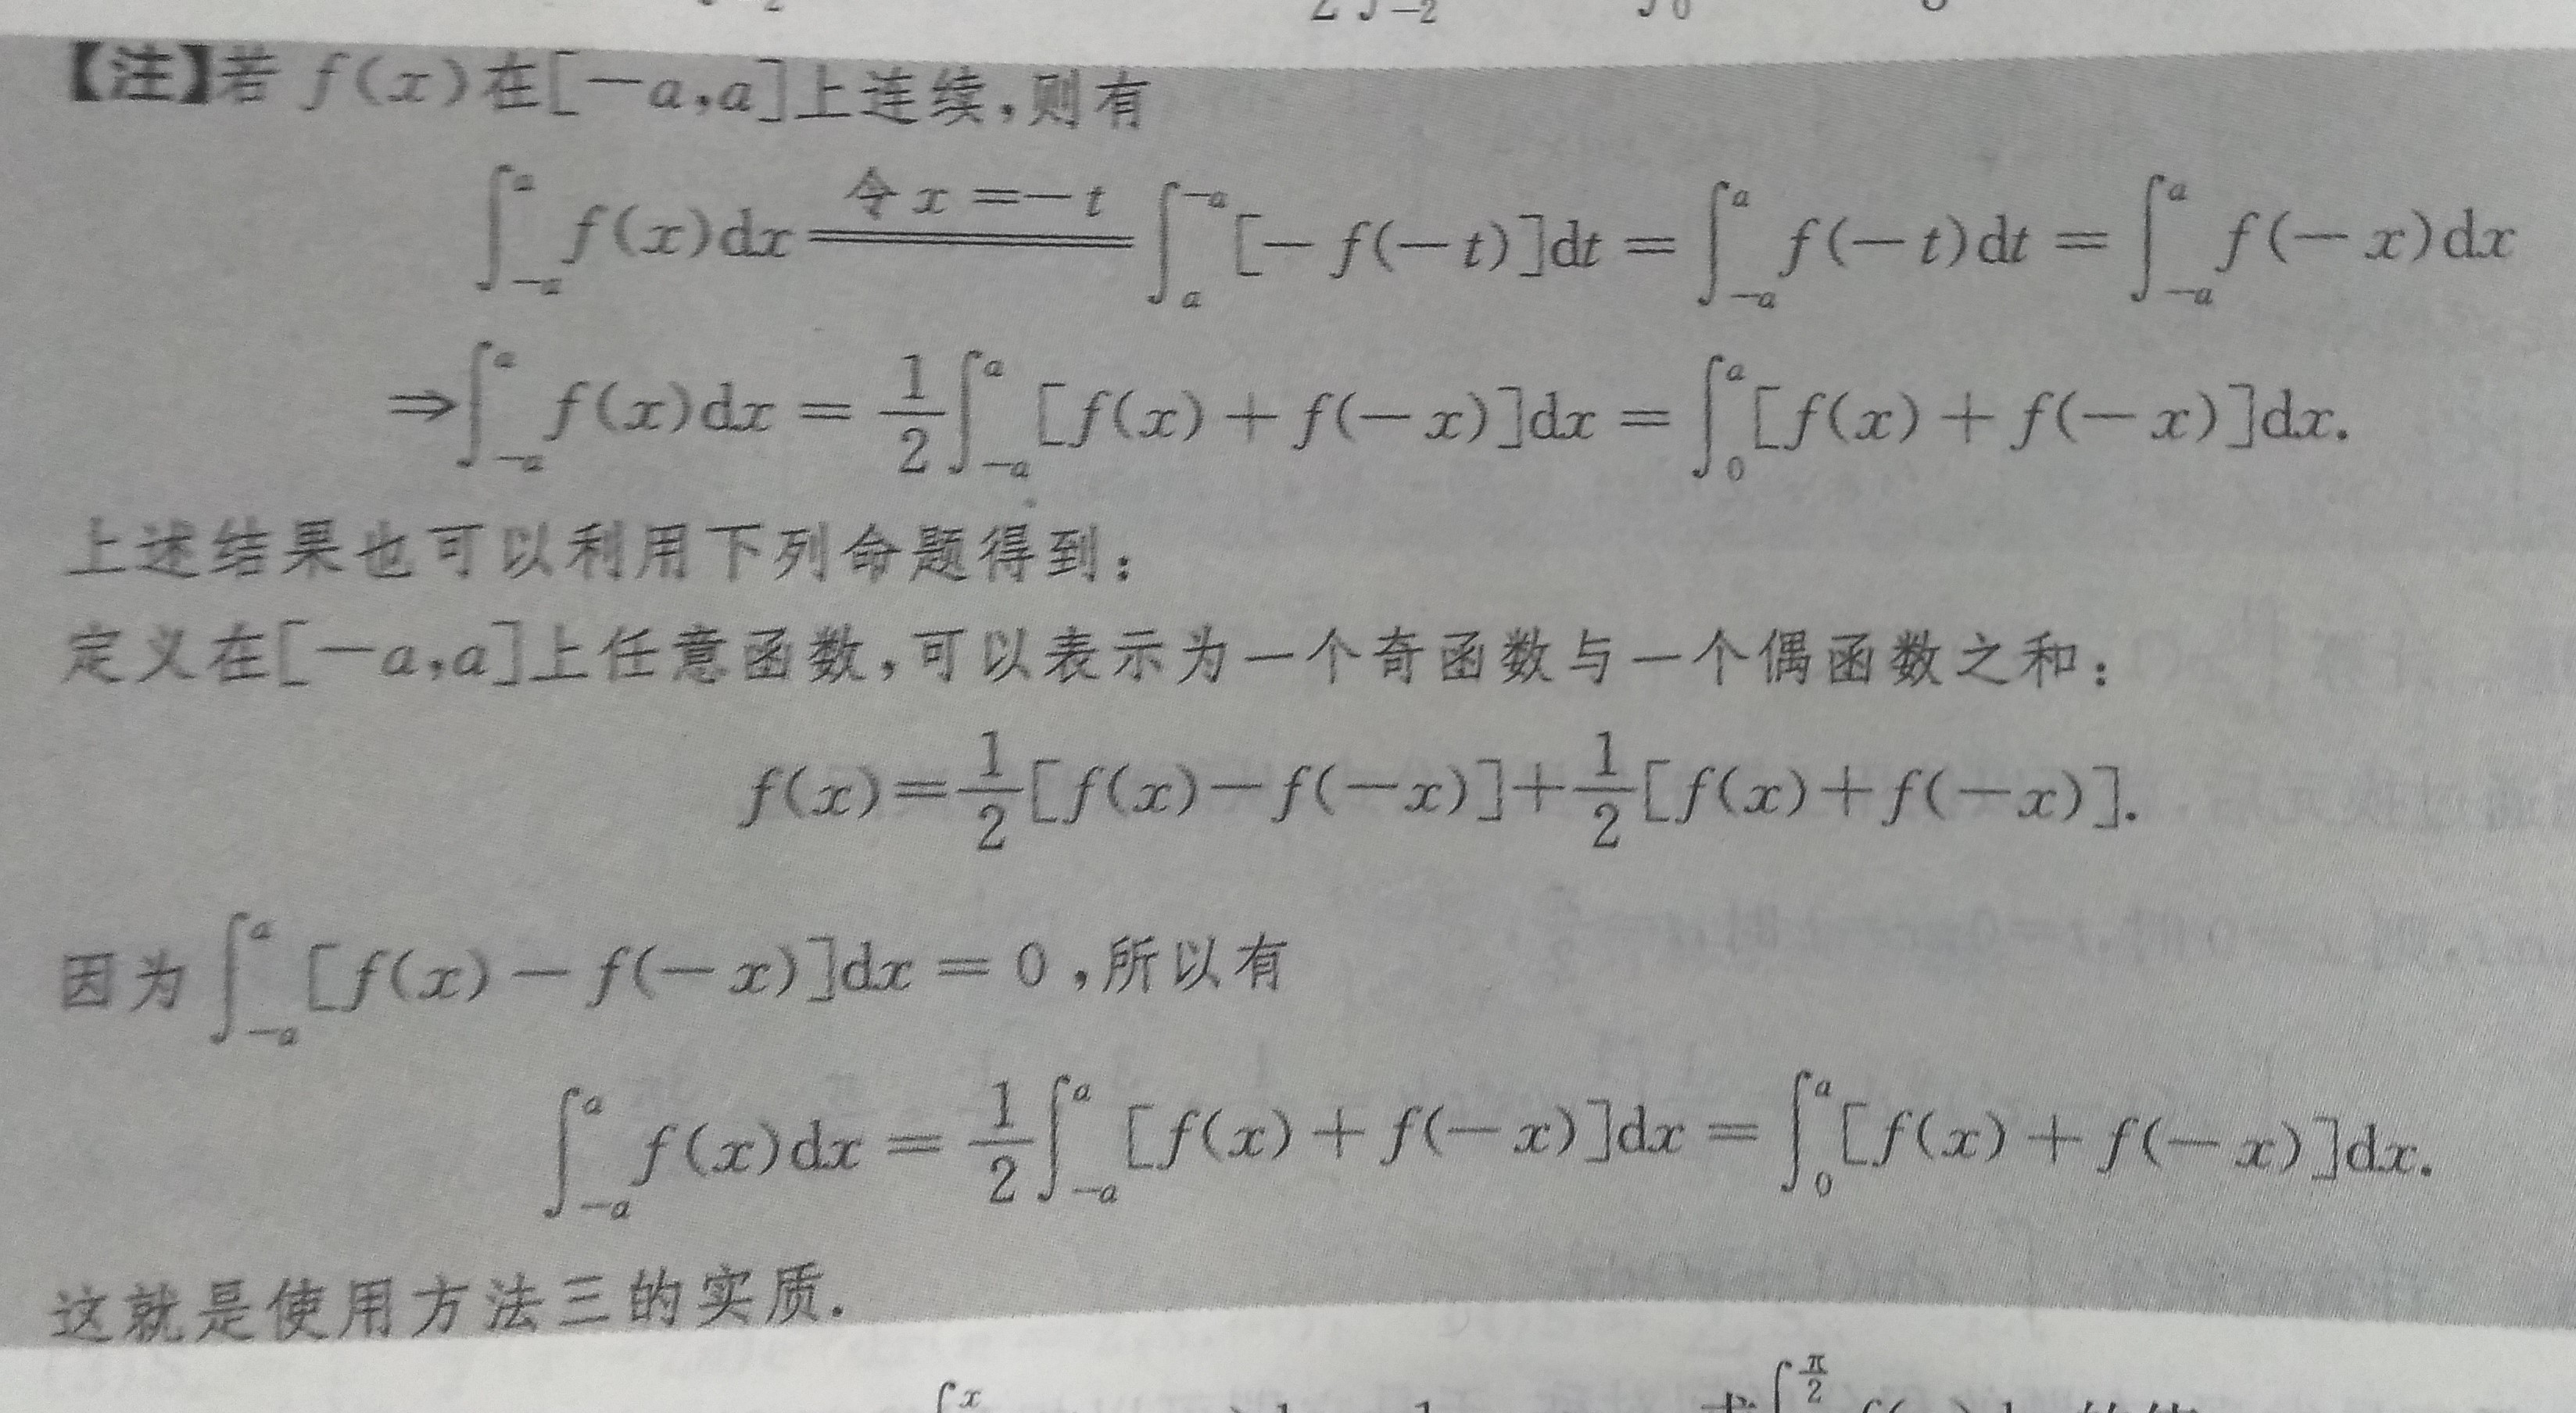
\includegraphics[width=13cm]{9345E7/2002379869.jpg}

\section{极值判定充分条件}
$f '(x_0)$左右异号 $\rightarrow$ 极值点

\begin{align}
&f'=0 \\
&f''(x_0) \neq 0
\end{align}
$\rightarrow$ 极值点

当$ f^{(n)} (x_0) \neq 0$ \\
1. n为偶   \\
    $f^{(n)} (x_0) \leq 0 \rightarrow $ 极大值  \\
    $f^{(n)} (x_0) \geq 0 \rightarrow $ 极小值  \\
    2. n为奇  \\
        拐点  \\

\section{多元函数极值与最值}
1. 二元函数取极值的必要条件
设z=f(x,y)在点($x_0,y_0$) \\
\begin{align}
&\mbox{一阶偏导数存在}\\
&\mbox{取极值}
\end{align}则,$ f_x' (x_0 , y_0)=0 , f_y' (x_0 , y_0)=0 $

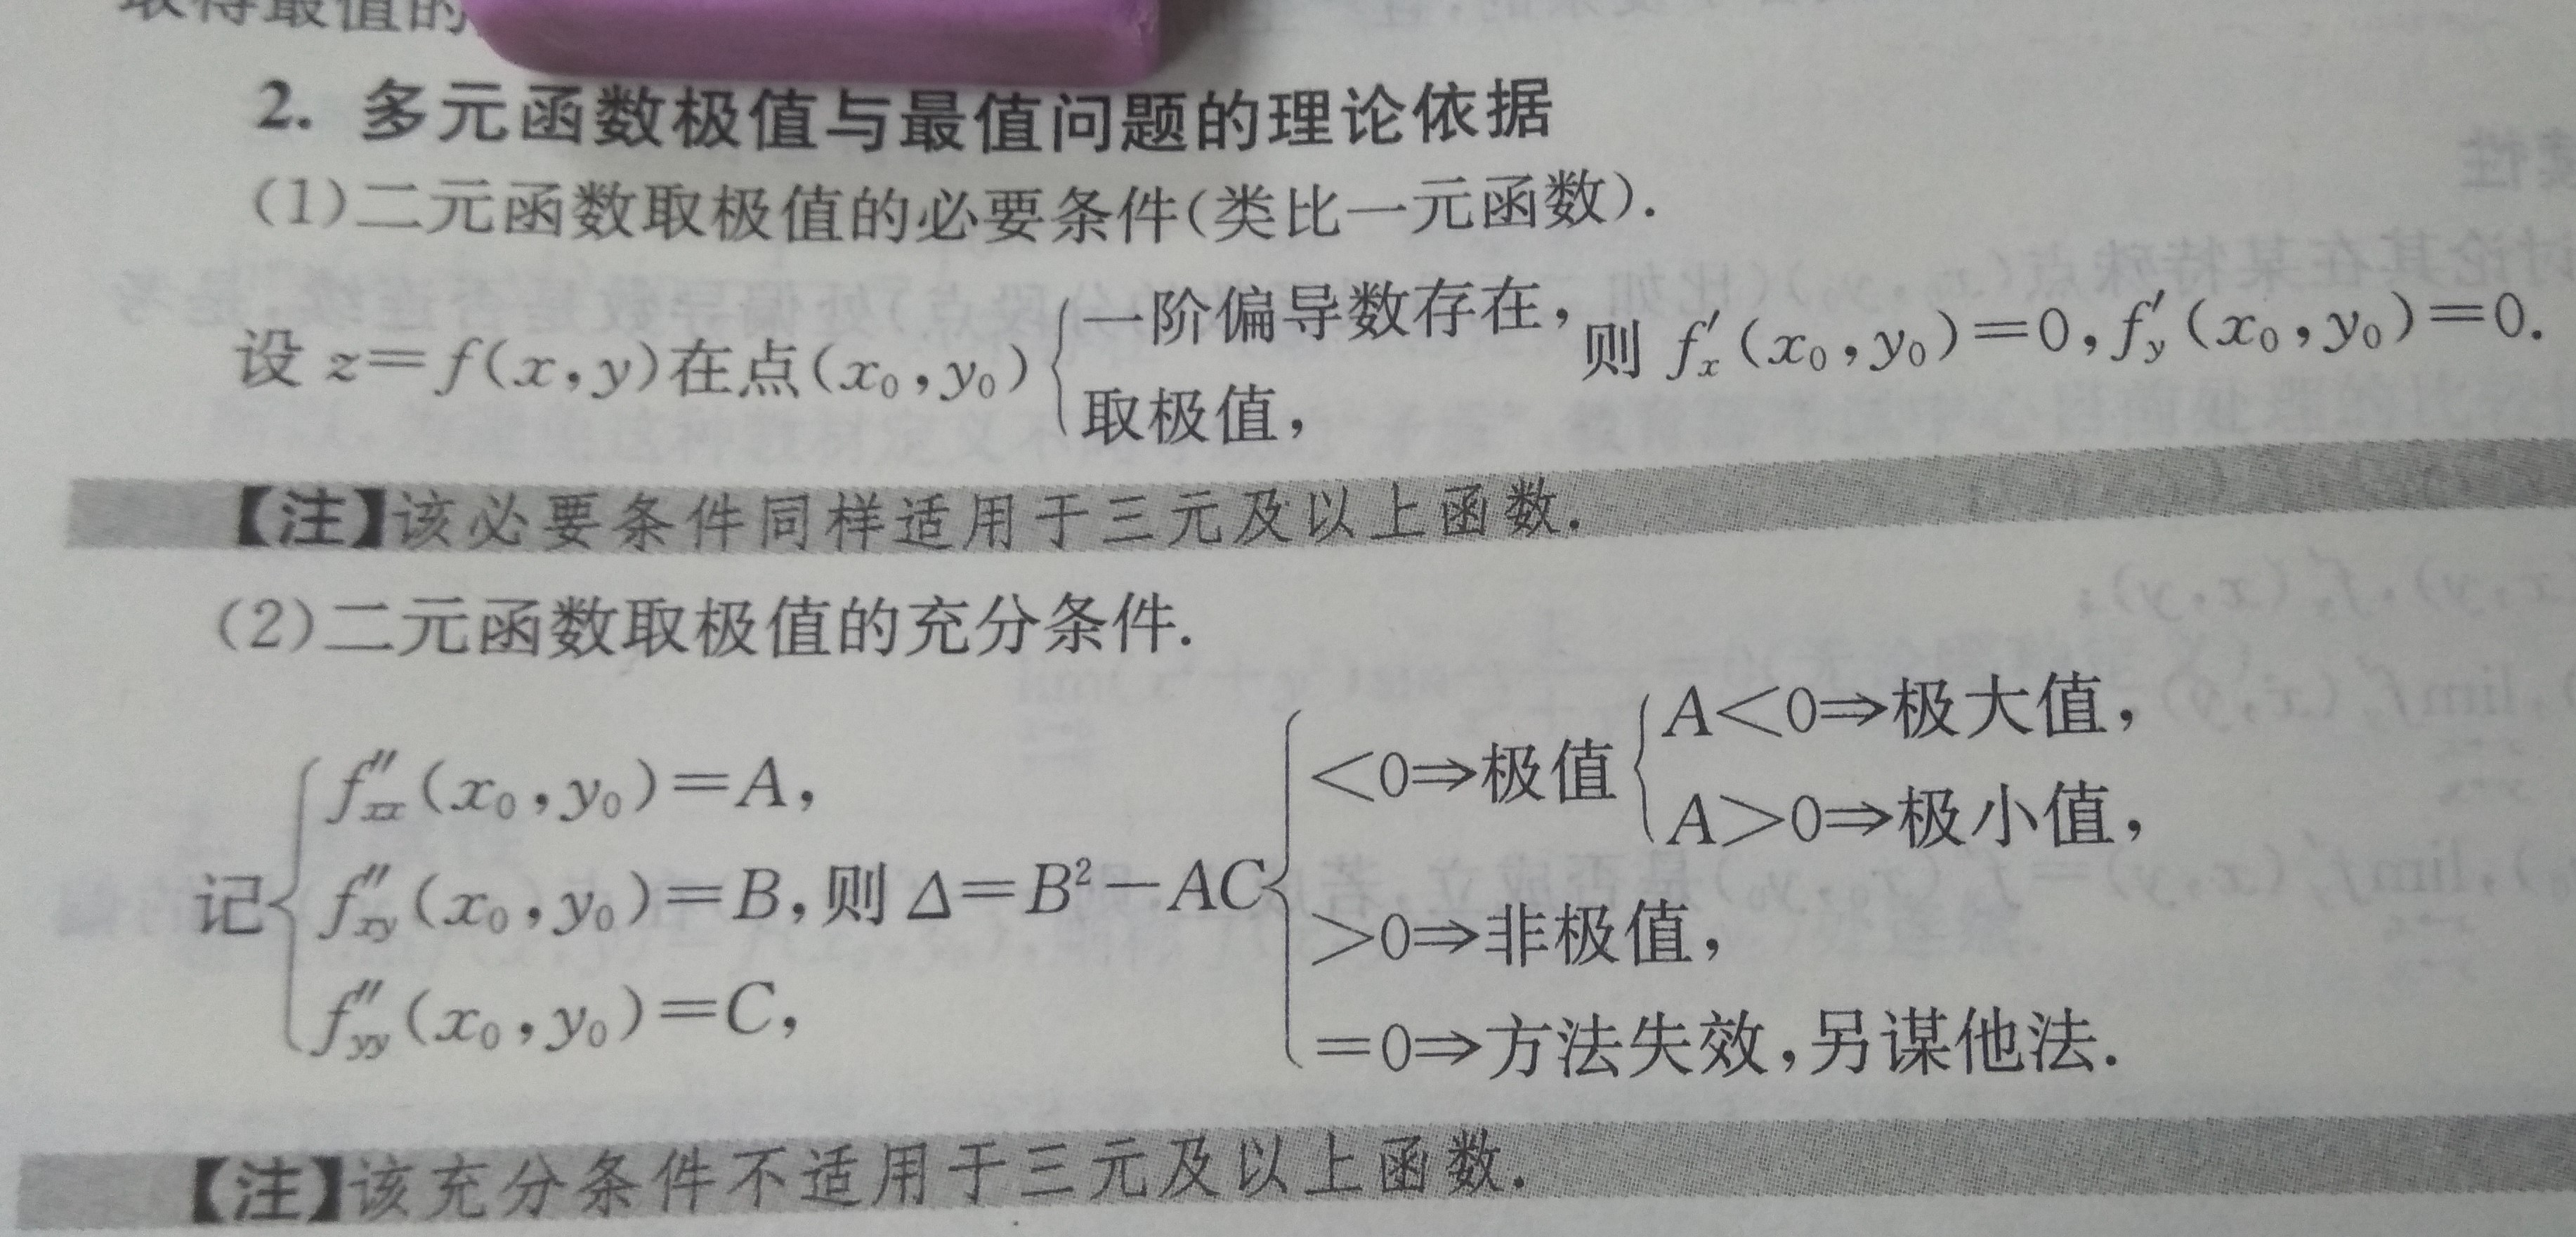
\includegraphics[width=13cm]{9345E7/2805530637.jpg}

\section{凹凸性定义}
    1. 凹  $ f(\frac{x_1+x_2}{2}) < \frac{f(x_1)+f(x_2)}{2}$   \\
    1. 凹  $ f[λx_1 +(1-λ)x_2] \leq λf(x_1)+(1-λ)f(x_2)$  \\

\section{极值点与拐点不要求导数存在}
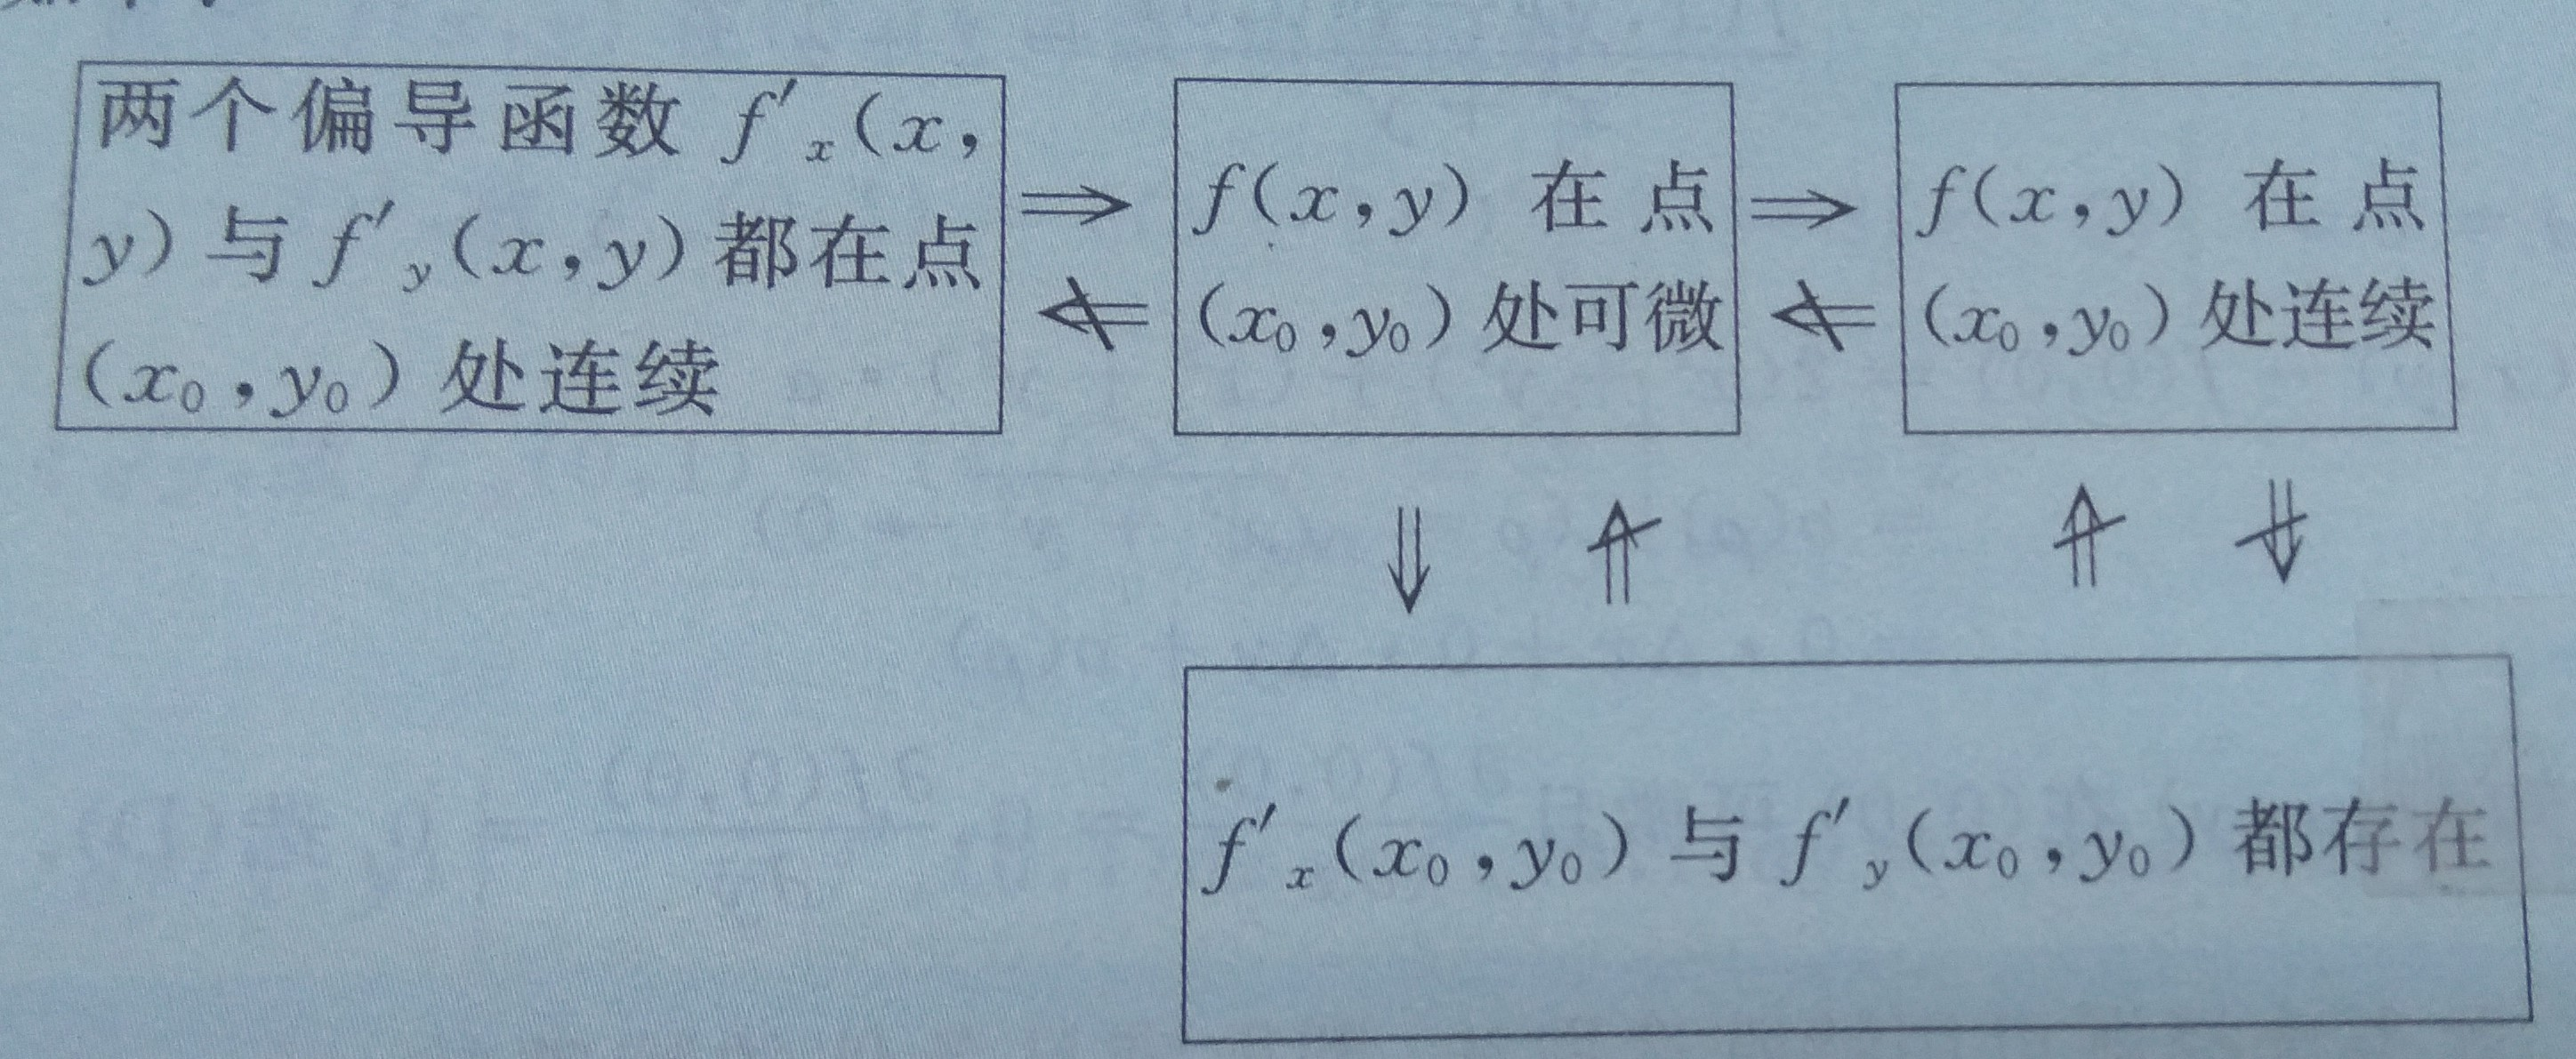
\includegraphics[width=13cm]{9345E7/2367085874.jpg}

\section{曲率半径}
$ k= \frac{|y''|}{{(1+y'^2)}^{3 \over 2}}$
R= $ \frac{1}{k}=\frac{{(1+y'^2)}^{3 \over 2}}{|y''|}$

\section{弧长}
L=$ \int_α^β \sqrt{r^2(θ)+[r'(θ)]^2}dθ$
\section{曲边扇形面积}
 S=$ \frac{1}{2} \int_α^β|r_1^2(θ)-r_2^2(θ)|dθ$

\section{极座标交换积分次续}
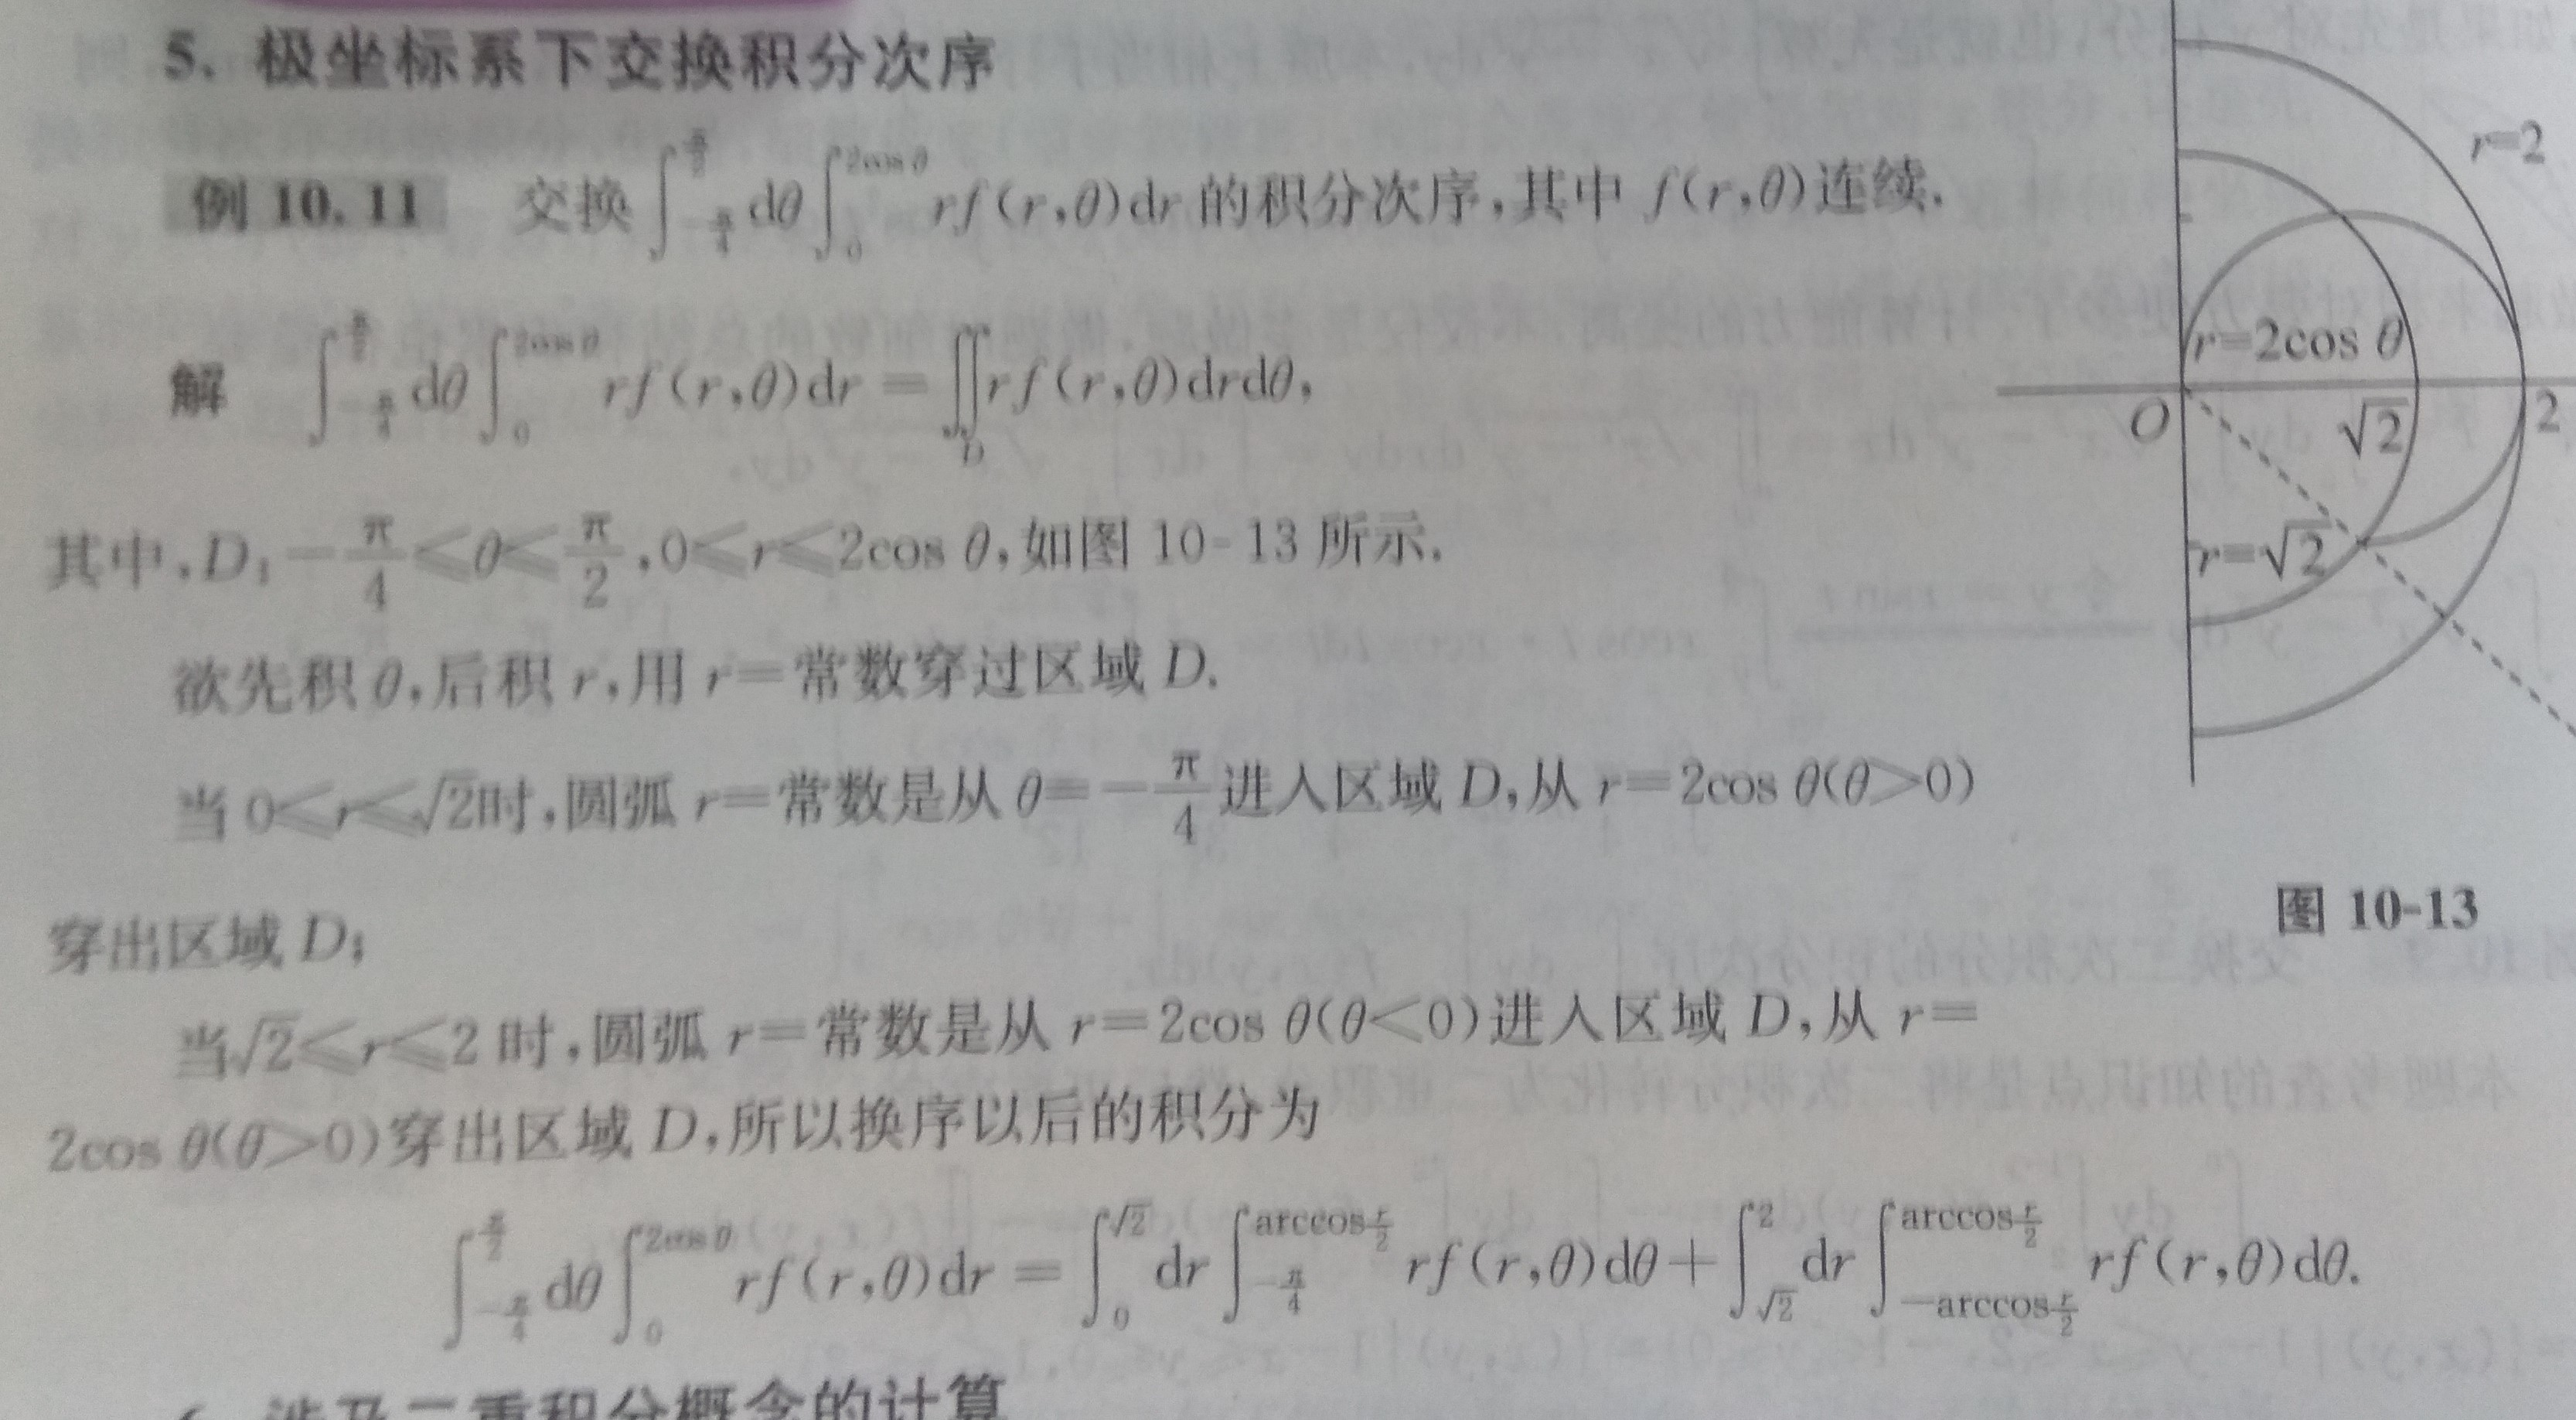
\includegraphics[width=13cm]{9345E7/3720754172.jpg}
\section{反常积分审敛}
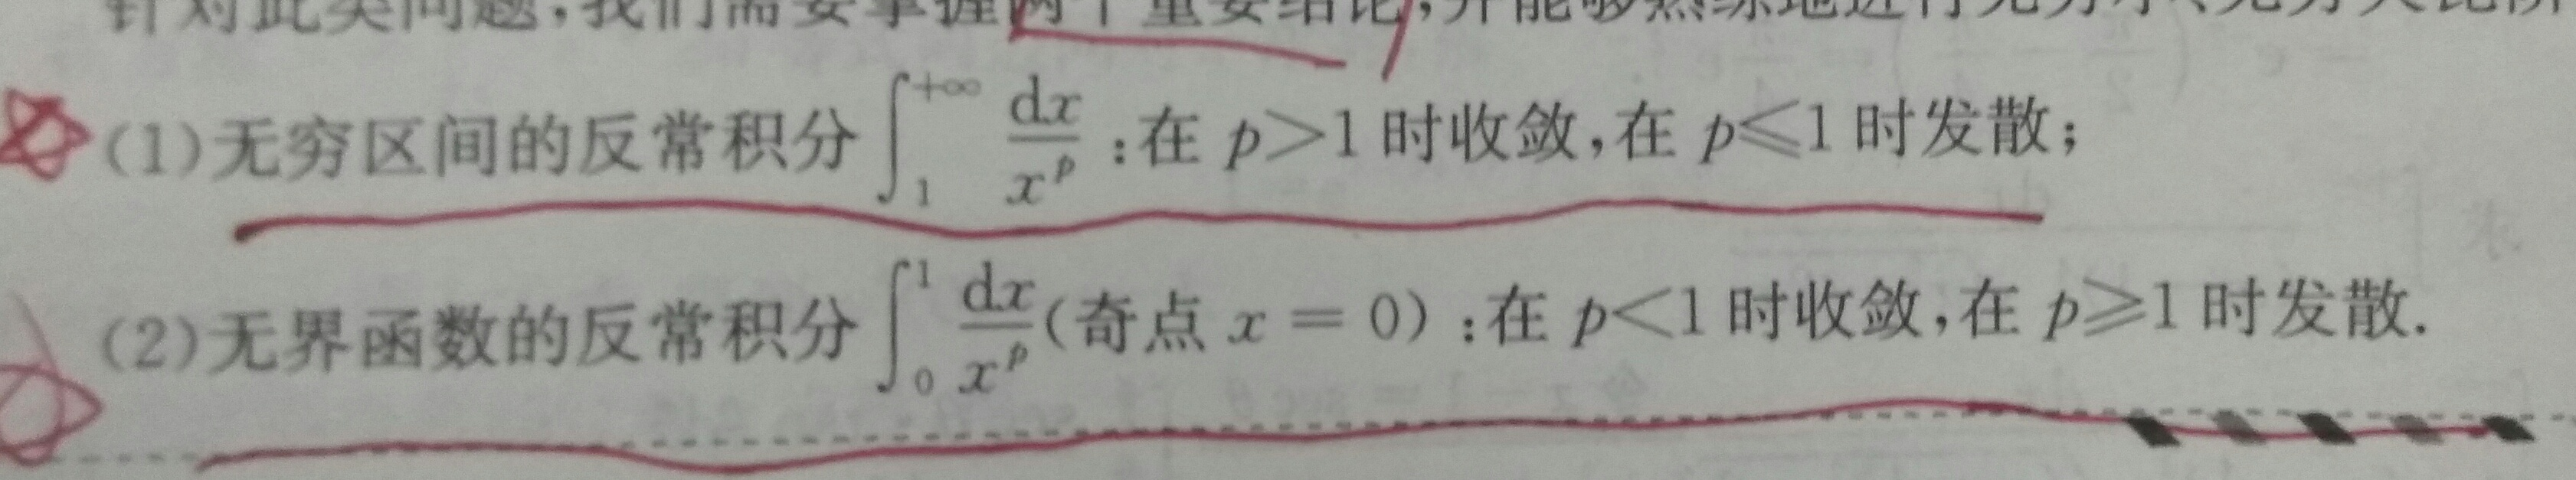
\includegraphics[width=13cm]{9345E7/2059466188.jpg}

\section{一阶微分方程}
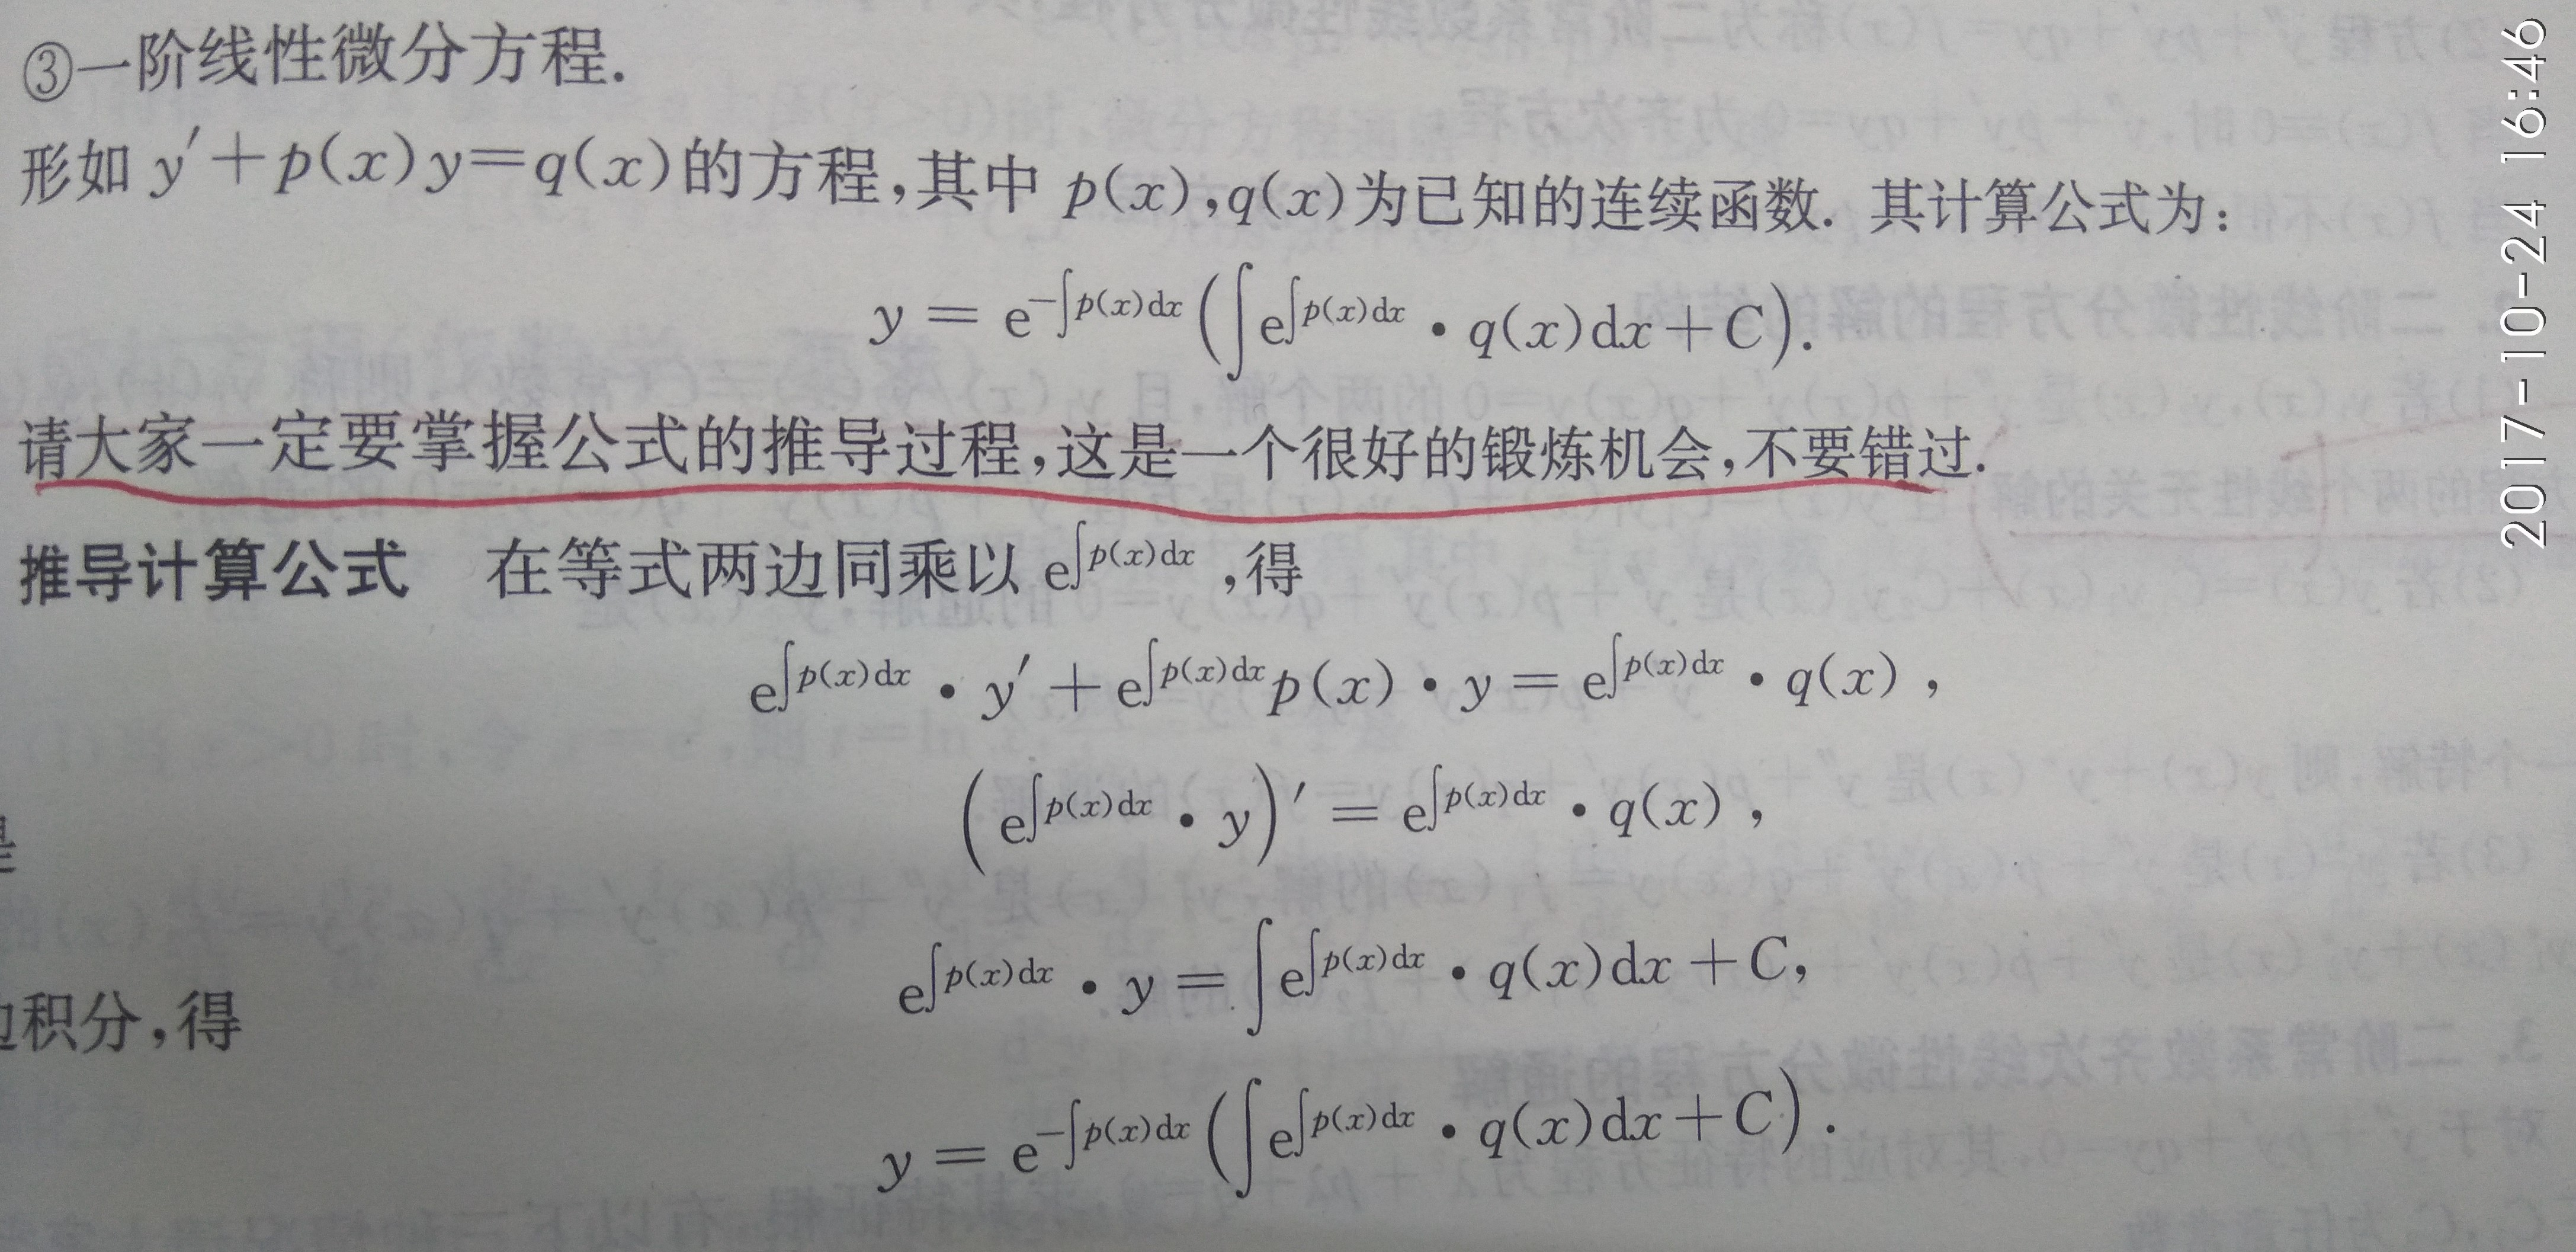
\includegraphics[width=13cm]{9345E7/677562795.jpg}

\section{一阶微分方程}
    当 $ u=\frac{y}{x} \Rightarrow y=ux\frac{dy}{dx}=u+x\frac{du}{dx}$
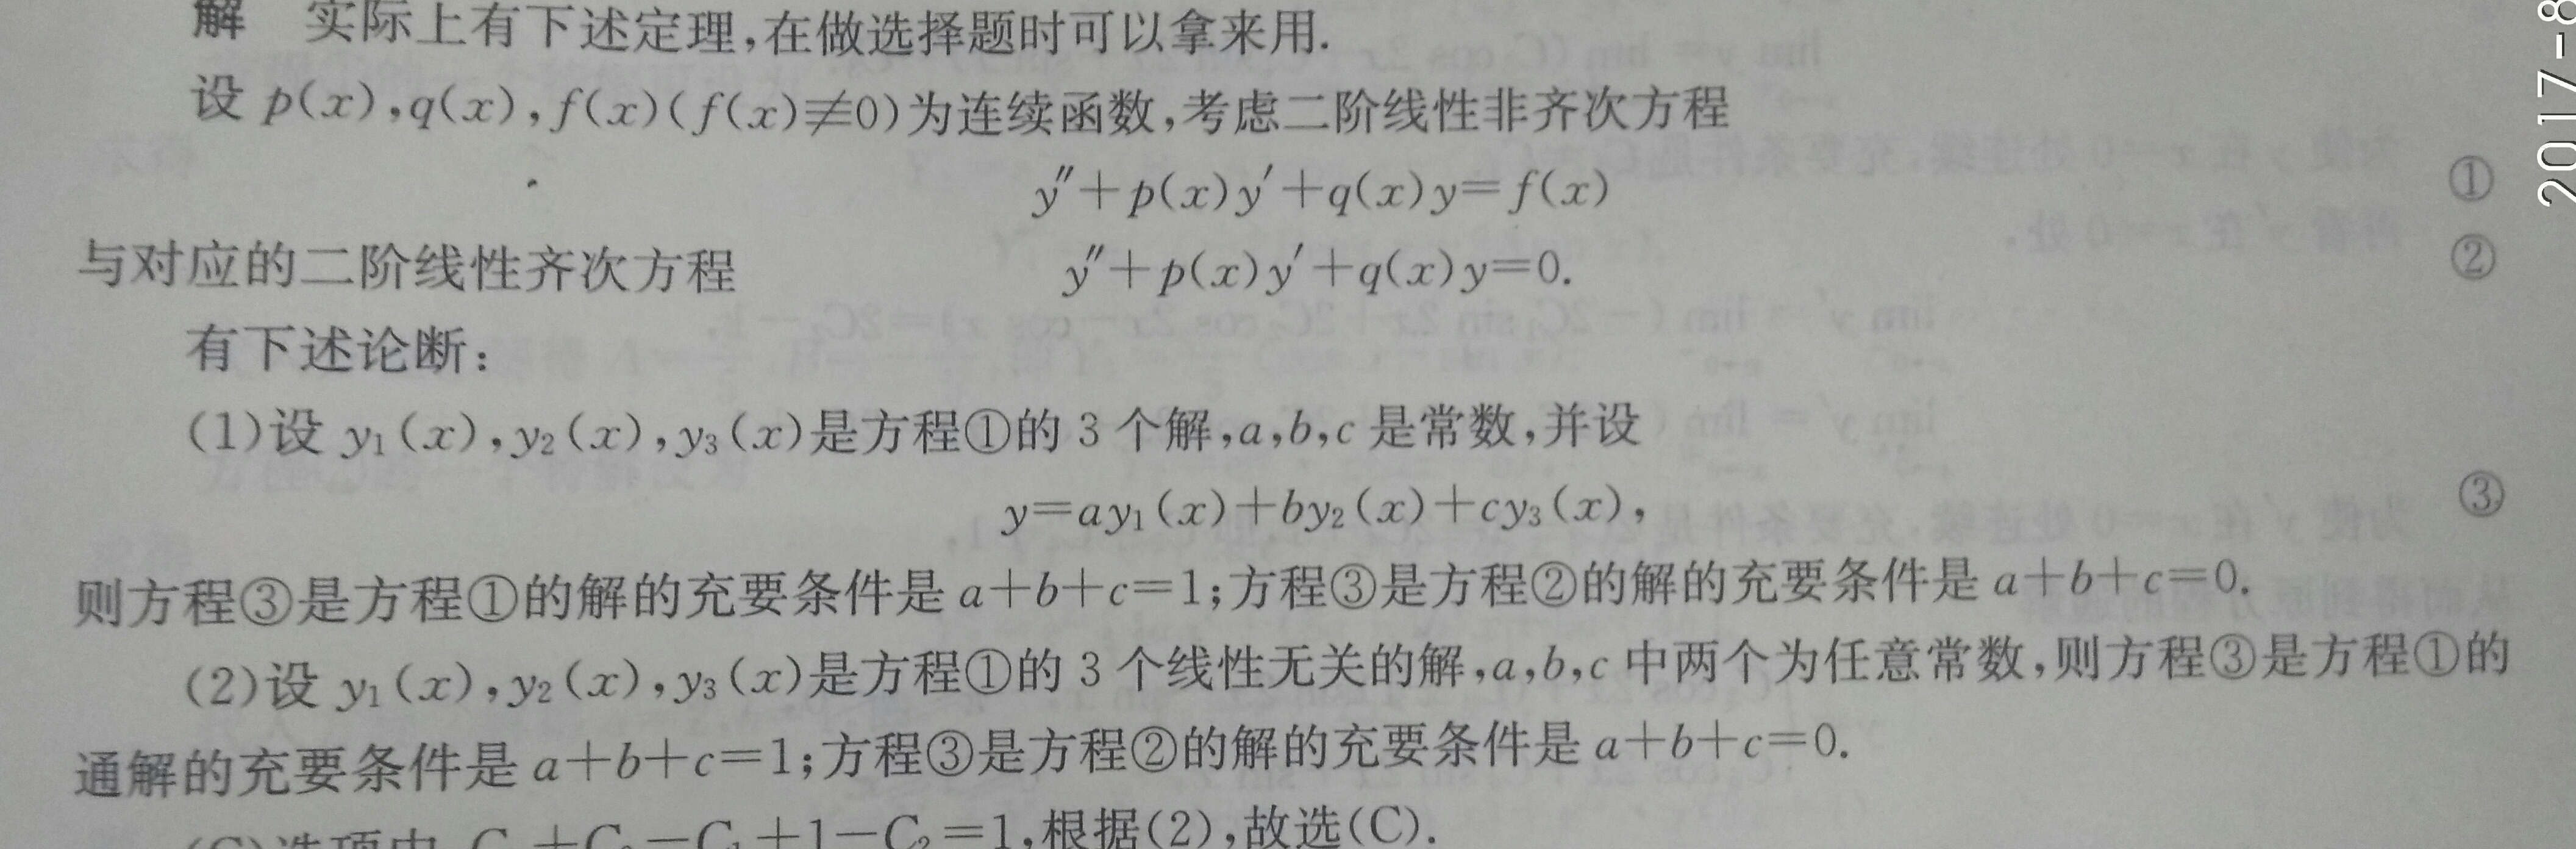
\includegraphics[width=13cm]{9345E7/478763472.jpg}
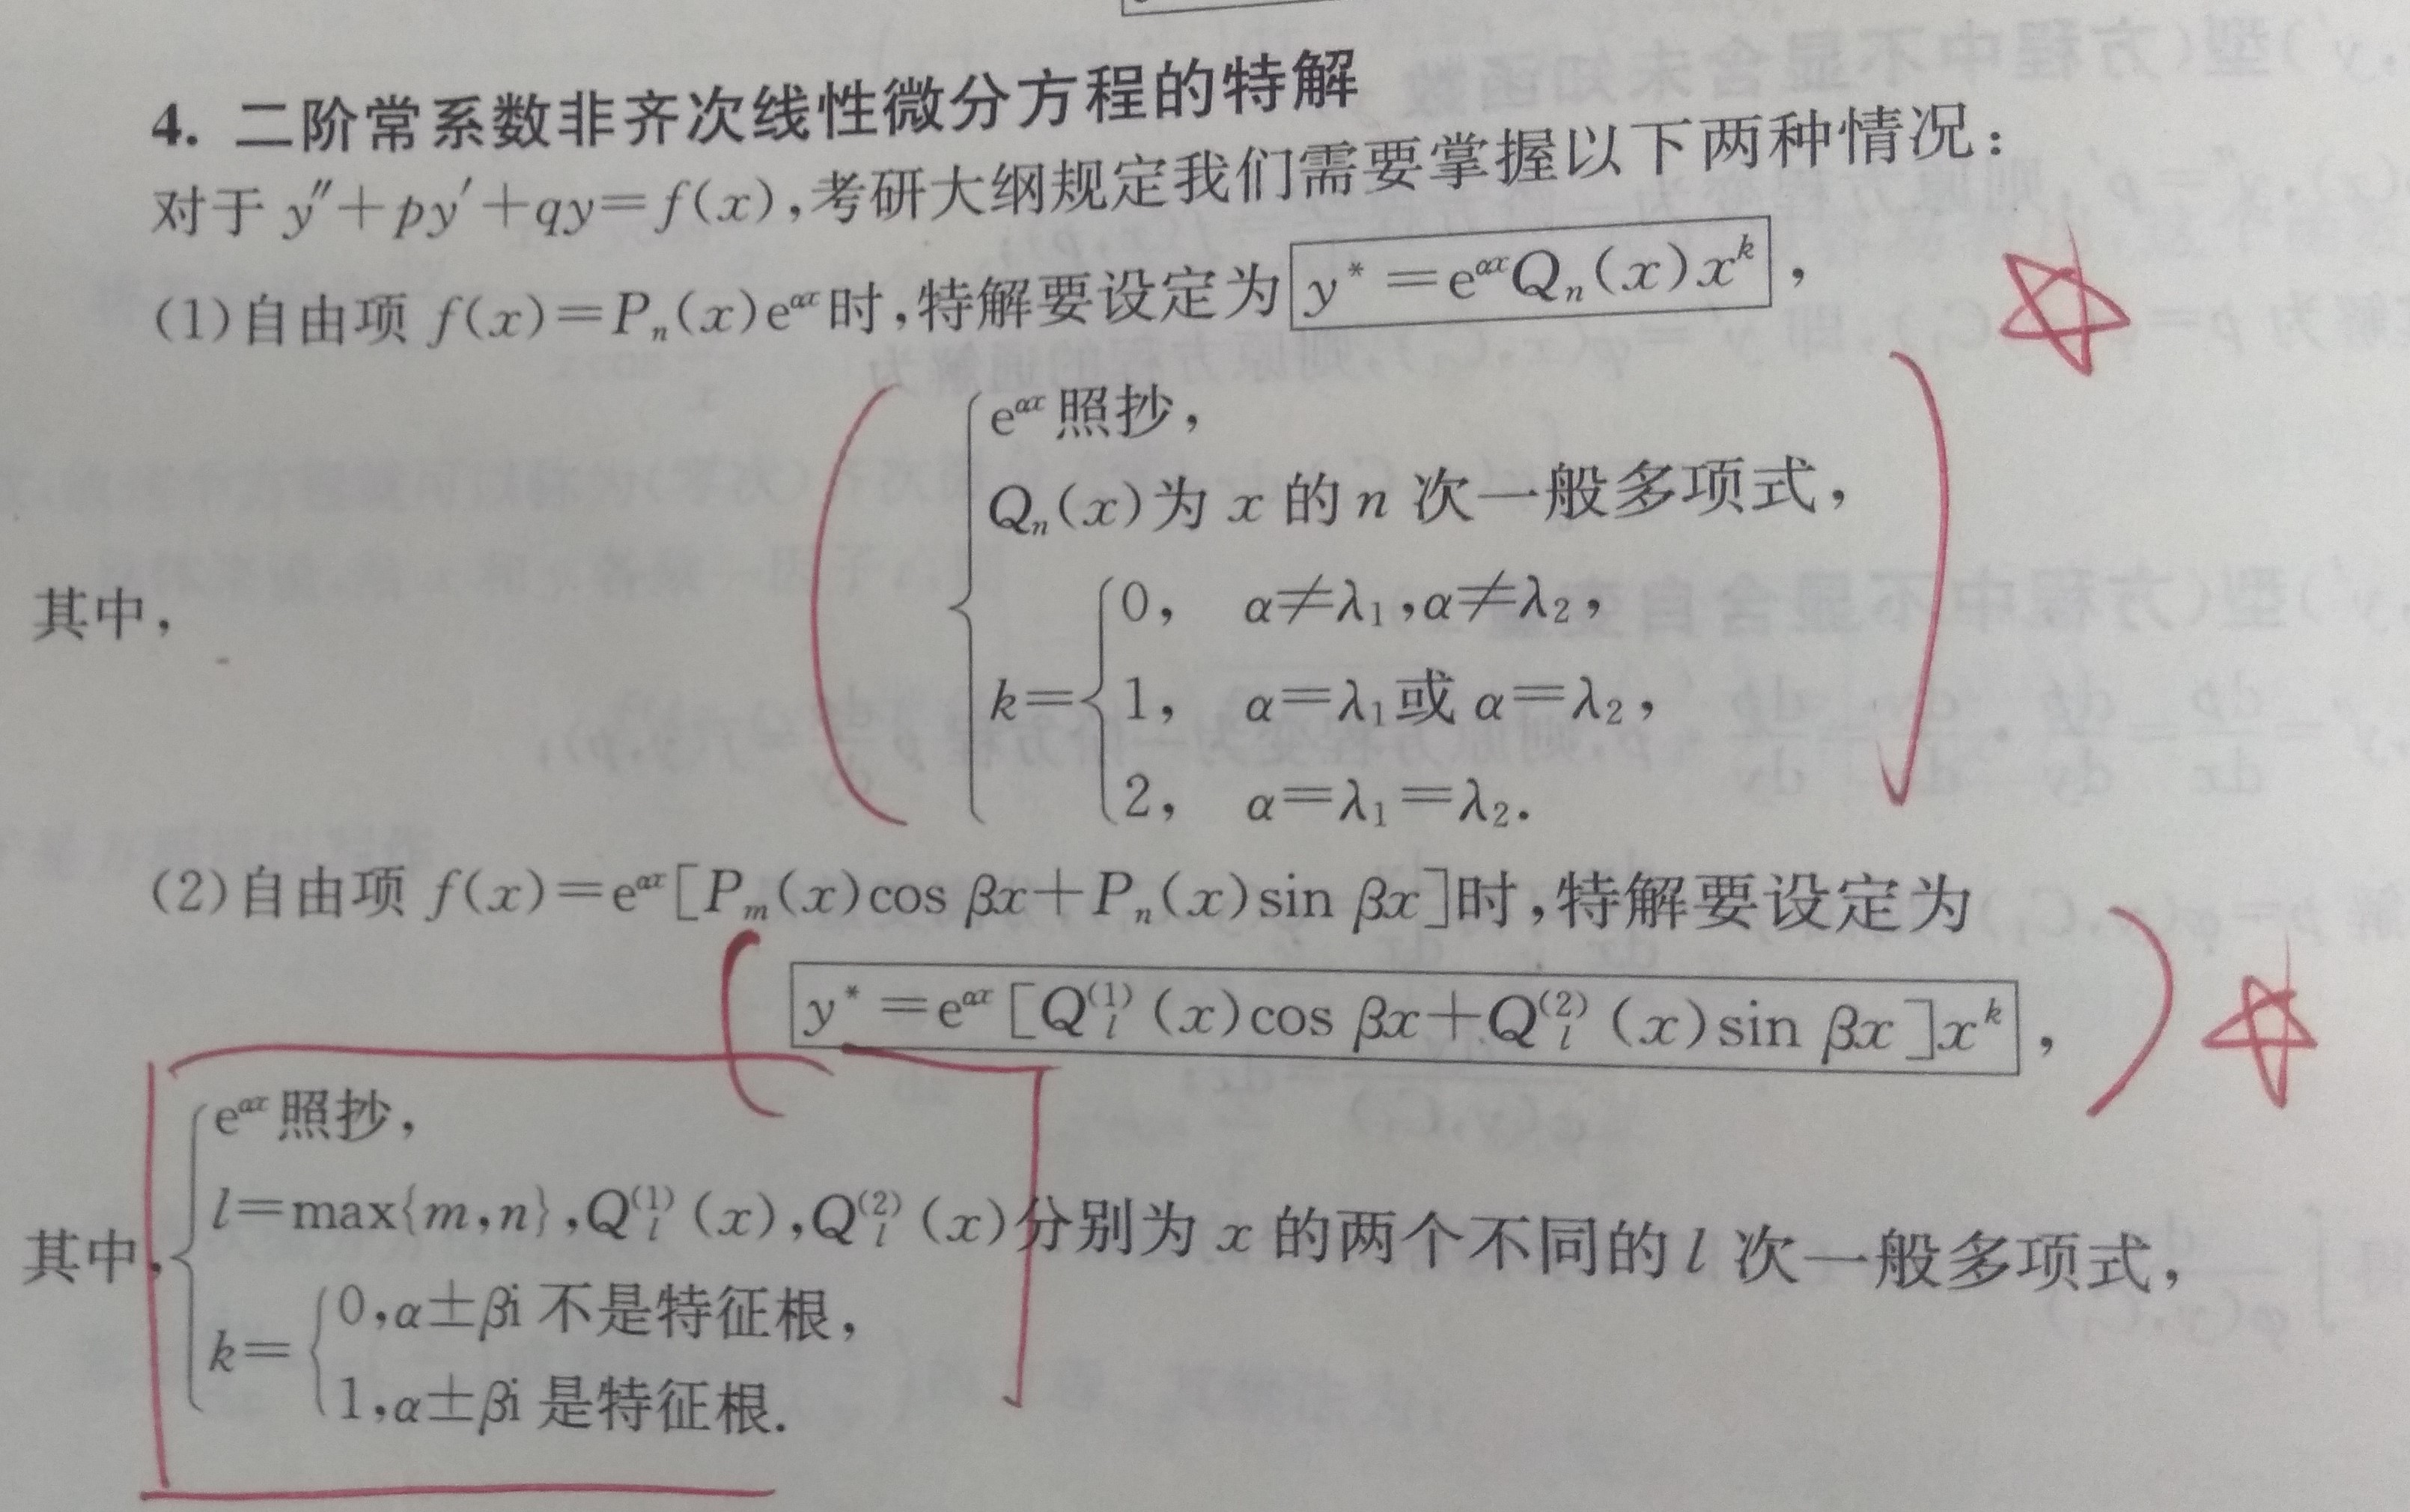
\includegraphics[width=13cm]{9345E7/595734581.jpg}
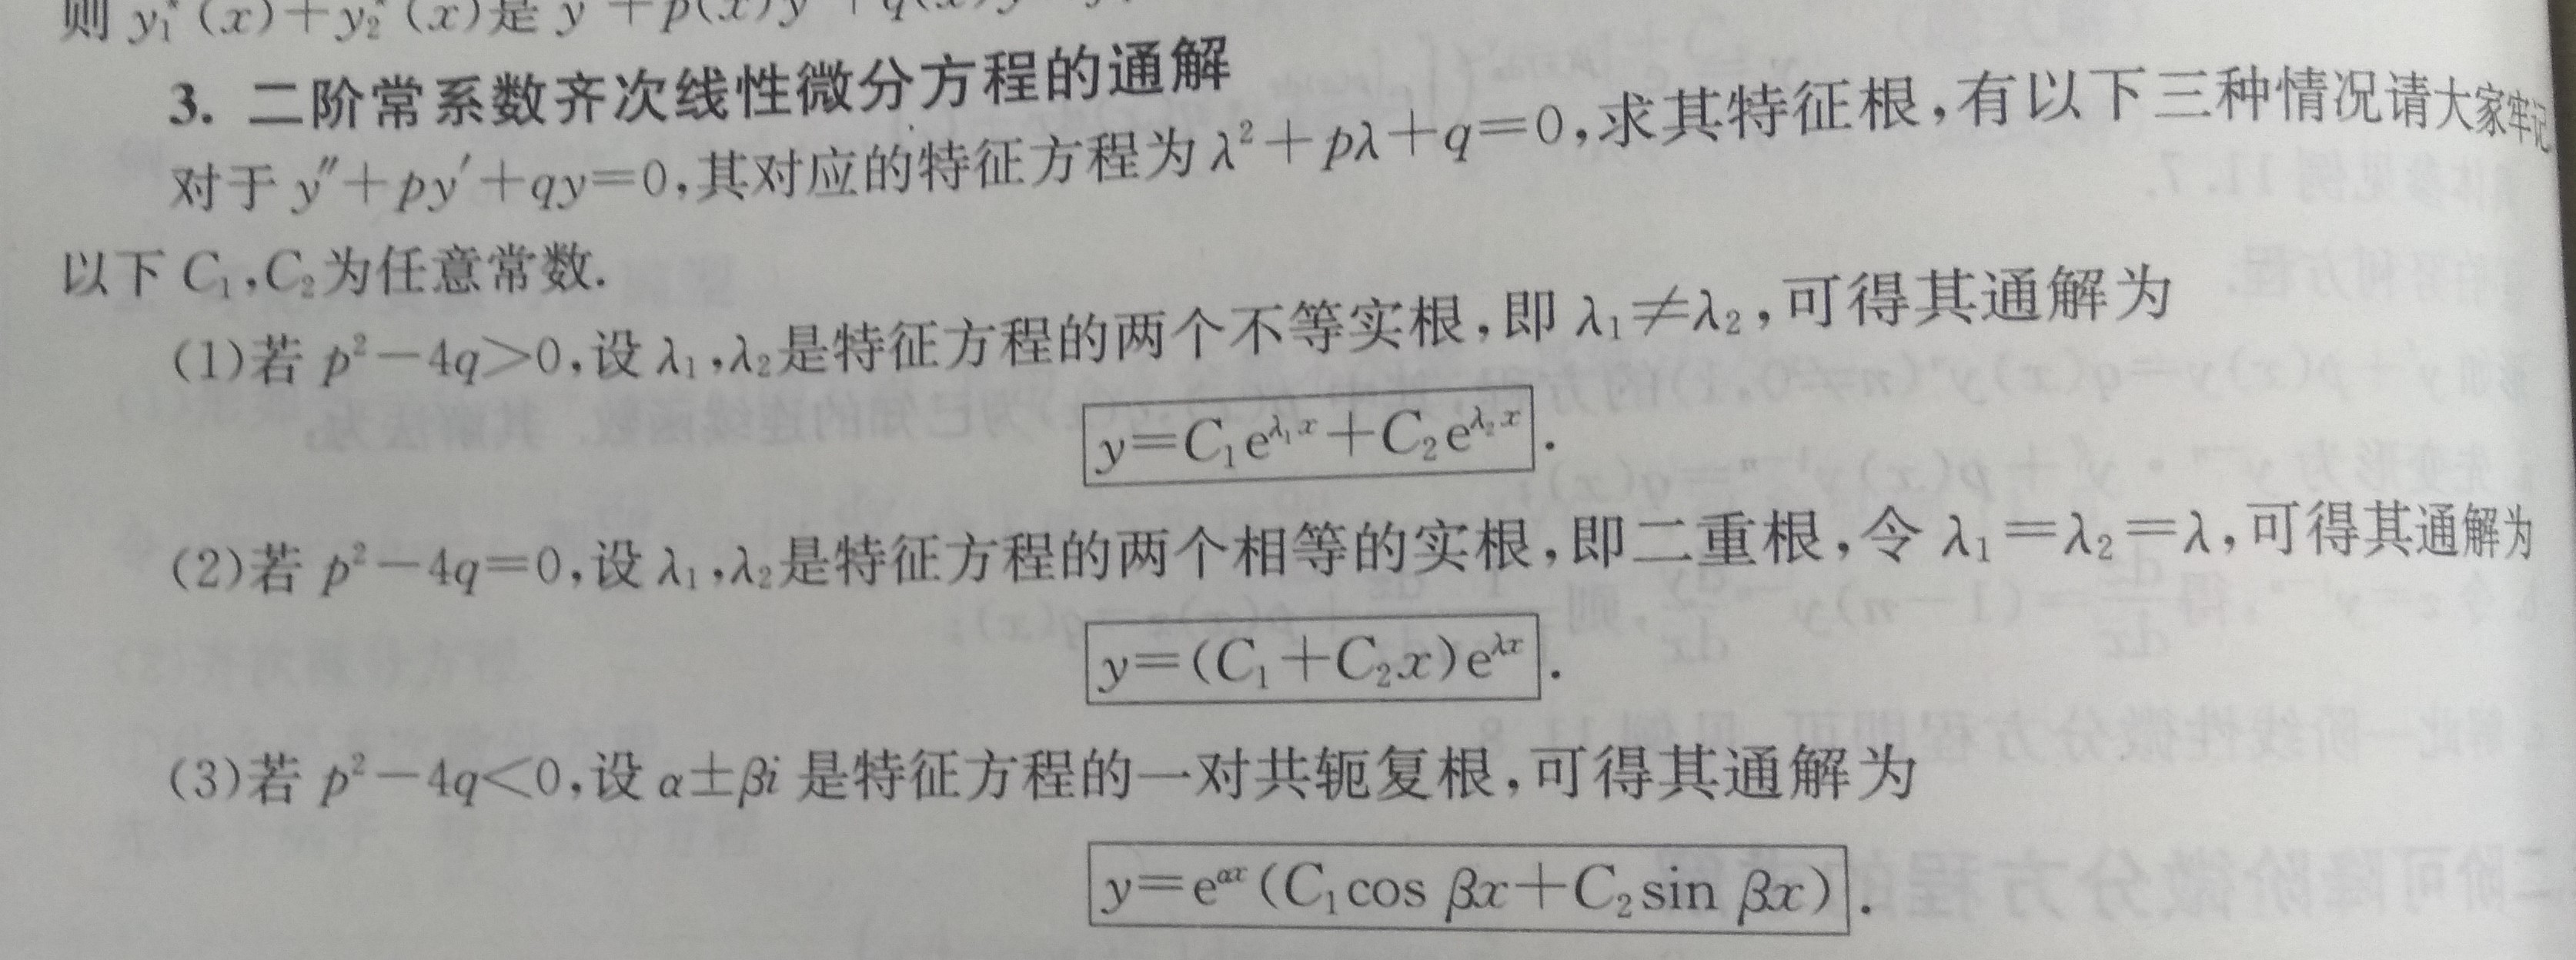
\includegraphics[width=13cm]{9345E7/601054614.jpg}








\end{document}
